\documentclass[12pt,reqno]{amsart}
%%%%%%%%%%%%%%%%%%%%%%%%%%%%%%%%%%%%%%%%%%%%%%%%%%%%%%%%%%%%%%%%%%%%%%%%%%%%%%%
%%%%%%%%%%%   PACKAGES %%%%%%%%%%%%%%%%%%%%%%%%%%%%%%%%%%%%%%%%%%%%%%%%%%%%%%%%
%%%%%%%%%%%%%%%%%%%%%%%%%%%%%%%%%%%%%%%%%%%%%%%%%%%%%%%%%%%%%%%%%%%%%%%%%%%%%%%

\usepackage[utf8]{inputenc}

%%---AMS packages---%% (automatically loaded in amsart or amsbook)
\usepackage{amsmath} %General package for maths (loads also amsbsy to make bold symbols)
\usepackage{amsthm} %Package for theorems
\usepackage{amssymb} %Symbols (loads also amsfonts)
\usepackage{amscd} %Package for rectangular diagrams
%\usepackage{amsrefs} %Gestió de referències


\usepackage{emptypage}
%\usepackage{pdfpages} %Include pdf documents

%\usepackage{dsfont} % Double stroke roman fonts
\usepackage{enumitem} %Enumerations
\usepackage{mathtools} %More symbols, etc.
\usepackage{mathrsfs} %Calligraphic symbols with \mathscr
%\usepackage{fancyhdr} %Customize the header
\usepackage{hyperref} %Makes references hyperlinks
\hypersetup{
	%true = make page number, not text, be link
    linktocpage = true,
    %set to all if you want both sections and subsections linked
    %linktoc=all,    
    colorlinks=true, 
    linkcolor=red,
} 
\usepackage{esint} %To write averaged integrals

%%%FIGURES AND IMAGES
\usepackage{graphicx} %For using \includegraphics
%\usepackage{wrapfig} %For figures wrapped inside the text
%\usepackage{float} %Interface for defining floating objects
%\usepackage{caption} %Customize the captions in floating environments
%\usepackage{subfigure}
%\usepackage{tcolorbox} %For boxing
%\tcbuselibrary{theorems}
%\tcbuselibrary{skins}

%\usepackage{pgf,tikz}
%\usepackage{mathrsfs}
%\usetikzlibrary{arrows}


%%%EDITION HELP
\usepackage[colorinlistoftodos]{todonotes} %Package to add TODO's in colors
\setlength{\marginparwidth}{2.3cm} % make todonotes appear wider
%\usepackage{showlabels} %Show the labels of equations and theorems
%\usepackage{showkeys} %Show the keys of all references
%\usepackage{refcheck}



%%%%%%%%%%%%%%%%%%%%%%%%%%%%%%%%%%%%%%%%%%%%%%%%%%%%%%%%%%%%%%%%%%%%%%%%%%%%%%%
%%%%%%%%%%%   THEOREM ENVIRONMENTS %%%%%%%%%%%%%%%%%%%%%%%%%%%%%%%%%%%%%%%%%%%%
%%%%%%%%%%%%%%%%%%%%%%%%%%%%%%%%%%%%%%%%%%%%%%%%%%%%%%%%%%%%%%%%%%%%%%%%%%%%%%%

\newtheorem{theorem}{Theorem}[section]
\newtheorem*{theorem*}{Theorem}
\newtheorem{proposition}[theorem]{Proposition}
\newtheorem{lemma}[theorem]{Lemma}
\newtheorem{corollary}[theorem]{Corollary}
\newtheorem{conjecture}[theorem]{Conjecture}

\theoremstyle{definition}
\newtheorem{definition}[theorem]{Definition}
\newtheorem{example}[theorem]{Example}

\theoremstyle{remark}
\newtheorem{remark}[theorem]{Remark}
\newtheorem*{remark*}{Remark}
\newtheorem{observation}[theorem]{Observation}

%%%%%%%%%%%%%%%%%%%%%%%%%%%%%%%%%%%%%%%%%%%%%%%%%%%%%%%%%%%%%%%%%%%%%%%%%%%%%%%
%%%%%%%%%%%   MACROS/ABREVIATIONS  %%%%%%%%%%%%%%%%%%%%%%%%%%%%%%%%%%%%%%%%%%%%
%%%%%%%%%%%%%%%%%%%%%%%%%%%%%%%%%%%%%%%%%%%%%%%%%%%%%%%%%%%%%%%%%%%%%%%%%%%%%%%

\newcommand{\con}[1]{\mathbb{#1}}
\newcommand{\C}{\con{C}} %Complex
\newcommand{\R}{\con{R}} %Real
\newcommand{\Q}{\con{Q}} %Rational
\newcommand{\Z}{\con{Z}} %Integer
\newcommand{\N}{\con{N}} %Natural
\newcommand{\T}{\con{T}} %Torus
\newcommand{\Sph}{\con{S}} %Sphere
\renewcommand{\H}{\con{H}}
\newcommand{\ccal}{\mathscr{C}}
\newcommand{\ecal}{\mathcal{E}}
\newcommand{\ical}{\mathcal{I}}
\newcommand{\lcal}{\mathcal{L}}
\newcommand{\ncal}{\mathcal{N}}
\newcommand{\ocal}{\mathcal{O}}
\newcommand{\ucal}{\mathcal{U}}

\makeatletter
\newcommand{\leqnomode}{\tagsleft@true\let\veqno\@@leqno}
\newcommand{\reqnomode}{\tagsleft@false\let\veqno\@@eqno}
\makeatother

\newcommand{\limn}{\displaystyle\lim_{n \rightarrow \infty}} %limit n to infinity
\newcommand{\norm}[1]{\left | \left |{#1} \right | \right |}
\newcommand{\seminorm}[1]{\left [ {#1} \right ] }
\newcommand{\laplacian}{\Delta}
\newcommand{\s}{\gamma}
\newcommand{\fraclaplacian}{(-\Delta)^\s}
\newcommand{\loc}{\mathrm{loc}}
\renewcommand{\d}{\,\mathrm{d}} %straight d with small space before
\newcommand{\dx}{\,\mathrm{d}x} %The usual differential of x
\newcommand{\ddt}[1][]{\dfrac{\d{#1}}{\d t}} %Derivative with respect t
\newcommand{\ddtpar}[1]{ \dfrac{\d}{\d t}\Big ( {#1} \Big)} %Derivative with respect t with parenthesis
\newcommand{\lp}[1]{\mathrm{L}^{#1}}%L^p spaces
\newcommand{\hp}[1]{\mathrm{H}^{#1}}%H^p spaces
\newcommand{\sobolev}[1]{\mathrm{W}^{#1}}%Sobolev spaces
\newcommand{\cp}[1]{\mathcal{C}^{#1}}%C^p spaces
\newcommand{\bpar}[1]{\left ( {#1}\right )}
\newcommand{\setcond}[2]{\left \{ #1 \ : \ #2  \right \}}
\newcommand\evalat[1]{_{\mkern1.5mu\big\vert_{\scriptstyle #1}}}
\newcommand{\normLinf}[1]{\left | \left |{#1} \right | \right |_{\lp{\infty}}}

%\newcommand{\averageline}{{\mathchoice 
%{\kern1ex\vcenter{\hrule height.4pt width 6pt depth0pt} \kern-9.3pt} {}
%{\kern1ex\vcenter{\hrule height.4pt width 4.3pt depth0pt} \kern-7pt} 
%{} {} }}
%\newcommand{\average}{\averageline \!\int}

\newcommand{\average}{\fint}

\newcommand\beqc[1]{\left\{\begin{array}{#1}}
\newcommand\eeqc{\end{array} \right.}
\def\PDEsystem{rcll}
\def\bmatrix{\begin{pmatrix}}
\def\ematrix{\end{pmatrix}}
\DeclareMathOperator{\Tr}{Tr}
\DeclareMathOperator{\tr}{tr}
\DeclareMathOperator{\Det}{Det}
\DeclareMathOperator{\dist}{dist}
\DeclareMathOperator{\diam}{diam}
\DeclareMathOperator{\sign}{sign}
\DeclareMathOperator{\sech}{sech}
\DeclareMathOperator{\PV}{P.V.}
\let\div\relax
\DeclareMathOperator{\div}{div}
\newcommand{\usub}{\underline{u}}
\newcommand{\usup}{\overline{u}}
\def\ds{\displaystyle}

%%%%%%%%%%%%%%%%%%%%%%%%%%%%%%%%%%%%%%%%%%%%%%%%%%%%%%%%%%%%%%%%%%%%%%%%%%%%%%%
%%%%%%%%%%% SETTINGS %%%%%%%%%%%%%%%%%%%%%%%%%%%%%%%%%%%%%%%%%%%%%%%%%%%%%%%%%%
%%%%%%%%%%%%%%%%%%%%%%%%%%%%%%%%%%%%%%%%%%%%%%%%%%%%%%%%%%%%%%%%%%%%%%%%%%%%%%%
\setlength{\textwidth}{155mm}
\setlength{\textheight}{210mm}
\oddsidemargin=5mm
\evensidemargin=5mm

\numberwithin{equation}{section}

\graphicspath {{Images/}}

%%%%%%%%%%%%%%%%%%%%%%%%%%%%%%%%%%%%%%%%%%%%%%%%%%%%%%%%%%%%%%%%%%%%%%%%%%%%%%%
%%%%%%%%%%% HYPHENATION %%%%%%%%%%%%%%%%%%%%%%%%%%%%%%%%%%%%%%%%%%%%%%%%%%%%%%%%%%
%%%%%%%%%%%%%%%%%%%%%%%%%%%%%%%%%%%%%%%%%%%%%%%%%%%%%%%%%%%%%%%%%%%%%%%%%%%%%%%
\hyphenation{auto-ma-ti-cally}

%%%%%%%%%%%%%%%%%%%%%%%%%%%%%%%%%%%%%%%%%%%%%%%%%%%%%%%%%%%%%%%%%%%%%%%%%%%%%%%
%%%%%%%%%%% GENERAL INFORMATION %%%%%%%%%%%%%%%%%%%%%%%%%%%%%%%%%%%%%%%%%%%%%%%
%%%%%%%%%%%%%%%%%%%%%%%%%%%%%%%%%%%%%%%%%%%%%%%%%%%%%%%%%%%%%%%%%%%%%%%%%%%%%%%

\title[Saddle solution to the fractional Allen-Cahn equation]{Uniqueness and stability of the saddle-shaped solution to the fractional Allen-Cahn equation}
\author{Juan-Carlos Felipe-Navarro} 
\address{J.C. Felipe-Navarro:
Universitat Polit\`ecnica de Catalunya and BGSMath, Departament de Matem\`{a}tiques, Diagonal 647, 08028 Barcelona, Spain}
\email{juan.carlos.felipe@upc.edu}

\author{Tomás Sanz-Perela}
\address{T. Sanz-Perela:
Universitat Polit\`ecnica de Catalunya and BGSMath, Departament de Matem\`{a}tiques, Diagonal 647, 08028 Barcelona, Spain}
\email{tomas.sanz@upc.edu}







\thanks{The first author is supported by MINECO grant MDM-2014-0445-16-4. The second author is supported by MINECO grant MDM-2014-0445. Both authors are supported by MINECO grants MTM2014-52402-C3-1-P and MTM2017-84214-C2-1-P, are members of the Barcelona Graduate School of Mathematics and part of the Catalan research group 2014 SGR 1083.}

\keywords{Fractional Allen-Cahn equation, saddle-shaped solution, Simons cone, nonlocal minimal surfaces, stability}




%%%%%%%%%%%%%%%%%%%%%%%%%%%%%%%%%%%%%%%%%%%%%%%%%%%%%%%%%%%%%%%%%%%%%%%%%%%%%%%
%%%%%%%%%%%%%%%%%%%%%%%%%%%%%%%%%%%%%%%%%%%%%%%%%%%%%%%%%%%%%%%%%%%%%%%%%%%%%%%
%%%%%%%%%%%%%%%%%%%%%%%%%%%%%%%%%%%%%%%%%%%%%%%%%%%%%%%%%%%%%%%%%%%%%%%%%%%%%%%
%%%%%%%%%%%%%%%%%%%%%%%%%%%%%%%%%%%%%%%%%%%%%%%%%%%%%%%%%%%%%%%%%%%%%%%%%%%%%%%
%%%%%%%%%%%%%%%%%%%%%%%%%%%%%%%%%%%%%%%%%%%%%%%%%%%%%%%%%%%%%%%%%%%%%%%%%%%%%%%
\begin{document}


%%%%%%%%%%%%%%%%%%%%%%%%%%%%%%%%%%%%%%%%%%%%%%%%%%%%%%%%%%%%%%%%%%%%%%%%%%%%%%%
%%%%%%%%%%%%%%%%%%%%%%%%%%%%%%%%%%%%%%%%%%%%%%%%%%%%%%%%%%%%%%%%%%%%%%%%%%%%%%%
\begin{abstract}
In this paper we prove the uniqueness of the saddle-shaped solution to the semilinear nonlocal elliptic equation $\fraclaplacian u = f(u)$ in $\R^{2m}$, where $f$ is of Allen-Cahn type. Moreover, we prove that this solution is stable if $2m\geq 14$. As a consequence of this result and the connection of the problem with nonlocal minimal surfaces, we show that the Simons cone $\setcond{(x', x'') \in \R^{m}\times \R^m}{|x'| = |x''|}$ is a stable nonlocal $(2\s)$-minimal surface in dimensions $2m\geq 14$.

Saddle-shaped solutions of the fractional Allen-Cahn equation are doubly radial, odd with respect to the Simons cone, and vanish only in this set. It was known that these solutions exist in all even dimensions and are unstable in dimensions $2$, $4$ and $6$. Thus, after our result, the stability remains an open problem only in dimensions $8$, $10$ and $12$.

The importance of studying this type of solution is due to its relation with the fractional version of a conjecture by De Giorgi. Saddle-shaped solutions are the simplest non 1D candidates to be global minimizers in high dimensions, a property not yet established in any dimension.
\end{abstract}
%%%%%%%%%%%%%%%%%%%%%%%%%%%%%%%%%%%%%%%%%%%%%%%%%%%%%%%%%%%%%%%%%%%%%%%%%%%%%%%
%%%%%%%%%%%%%%%%%%%%%%%%%%%%%%%%%%%%%%%%%%%%%%%%%%%%%%%%%%%%%%%%%%%%%%%%%%%%%%%


\maketitle




\section{Introduction}

This paper is devoted to the study of saddle-shaped solutions to the fractional Allen-Cahn equation
\begin{equation}
\label{Eq:AllenCahn}
\fraclaplacian u = f(u)  \quad \text{ in } \R^{n}\,,
\end{equation}
where $n=2m$ is an even integer, $f$ is of bistable type (see \eqref{Eq:fHypotheses} below), and $\fraclaplacian$ is the fractional Laplacian, defined for $\s\in(0,1)$ by
$$
\fraclaplacian u (x):= c_{n,\s}  \PV \int_{\R^{n}} \dfrac{u(x) - u(\overline{x})}{|x-\overline{x}|^{n+2\s}} \d \overline{x}\,.
$$
Here $c_{n,\s}>0$ is a normalizing constant depending only on $n$ and $\s$, and $\PV$ stands for principal value. This problem is motivated by the fractional De Giorgi conjecture and it is closely related to the theory of nonlocal minimal surfaces, as we will explain later in this introduction.

Throughout the paper we assume that $f\in C^{2,\alpha}\big((-1,1)\big)$, for some $\alpha\in (0,1)$, and that is of bistable type, i.e.,
\begin{equation}\label{Eq:fHypotheses}
f \text{ is odd, }\; f(0)=f(1)=0,\text{ and }
f''<0 \text{ in } (0,1).
\end{equation}
Note that as a consequence we have $f>0$ in $(0,1)$. A typical example of this kind of nonlinearity is $f(u)=u-u^3$.

An important role in this paper is played by the Simons cone, which is defined in $\R^{2m}$ by
$$
\mathscr{C} = \setcond{x = (x', x'') \in \R^{m}\times \R^m}{|x'| = |x''|}\,.
$$
It is well known that the Simons cone has zero mean curvature at every point $x \in \ccal \setminus \{0\}$, in every dimension $2m \geq 2$. However, it is only in dimensions $2m \geq 8$ that $\ccal$ is a minimizer of the area functional, as established by Bombieri, De Giorgi, and Giusti in \cite{BombieriDeGiorgiGiusti}. Regarding the fractional setting, for every $\s\in(0,1/2)$, $\ccal$ has zero \emph{nonlocal} mean curvature in every even dimension but it is not known if, in addition,  it is a minimizer of the fractional perimeter in dimensions $2m\geq 8$. We recall that it is only in dimension $2m=2$ where we have a complete classification of minimizing nonlocal minimal cones (see \cite{SavinValdinoci-Cones}). The only other result concerning the possible stability of the Simons cone is established in \cite{DaviladelPinoWei} by Dávila, del Pino, and Wei. In that paper, the authors find a remarkable stability criterion for Lawson cones consisting of an inequality involving hypergeometric quantities depending on $\s$ and the dimension $n$. Although such criterion has not been checked analytically (probably a hard task), it can be verified numerically. With a numerical computation, \cite{DaviladelPinoWei} shows that, in dimensions $n \leq 6$ and for $\s $ close to zero, no Lawson cone with zero nonlocal mean curvature is stable. The Simons cone is a particular case of Lawson cone corresponding to $C_m^m(1)$ in the notation of \cite{DaviladelPinoWei}. Numerics also shows that all Lawson cones in dimension $7$ are stable if $\s$ is close to zero. These results for small $\s$ fit with the general belief that, in the fractional setting, the Simons cone should be stable (and even a minimizer) in dimensions $2m \geq 8$ (as in the local case), probably for all $\s\in(0,1/2)$, though this is still an open problem. 

In the present paper, we make a first contribution to the previous question by showing that the Simons cone is a stable $(2\s)$-minimal cone in dimensions $2m\geq 14$. Our proof uses the so-called saddle-shaped solution to the Allen-Cahn equation. As we will see in more detail, by the fractional Modica-Mortola type $\Gamma$-convergence result, the remarks above on the stability of the Simons cone are expected to hold also for saddle-shaped solutions. Indeed, our proof proceeds by establishing the stability of such solution to the fractional Allen-Cahn equation in dimensions $2m \geq 14$ (see Theorem~\ref{Thm:Stability} below). Then, as a consequence of this and a recent result by Cabré, Cinti, and Serra in \cite{CabreCintiSerra-Stable} (see also the comments in \cite{CabreCintiSerra-Cones}) concerning the preservation of stability along a blow-down procedure for the fractional Allen-Cahn equation, we deduce the stability of the Simons cone as a nonlocal minimal surface in these dimensions (see Corollary~\ref{Cor:SimonsConeStableDim14}). 

To introduce saddle-shaped solutions, we define the following variables:
$$
s = \sqrt{x_1^2 + \ldots + x_m^2 } \quad \text{ and } \quad 
t = \sqrt{x_{m+1}^2 + \ldots + x_{2m}^2}\,,
$$
for which the Simons cone becomes $\mathscr{C} = \{s=t\}$.
Through the paper we will also use the letter $\ocal$ to denote one side of the cone:
$$
\ocal:= \setcond{x = (x', x'') \in \R^{m}\times \R^m}{|x'| > |x''|} = \{s > t\}.
$$

We define saddle-shaped solutions as follows.

\begin{definition}
\label{Def:SaddleShapedSol}
We say that a bounded solution $u$ to \eqref{Eq:AllenCahn} is a \emph{saddle-shaped solution} (or simply \emph{saddle solution}) if
\begin{enumerate}[label=(\roman{*})]
\item $u$ is a doubly radial function, that is, $u = u(s,t)$.
\item $u$ is odd with respect to the Simons cone, that is, $u(s,t)=-u(t,s)$.
\item $u > 0$ in $\ocal$.
\end{enumerate}
\end{definition}

Saddle-shaped solutions for the classical Allen-Cahn equation involving the Laplacian were first studied by Dang, Fife, and Peletier in \cite{DangFifePeletier} in dimension $2m=2$. They established the existence and uniqueness of this type of solutions, as well as some monotonicity properties and asymptotic behavior. In \cite{Schatzman}, Schatzman studied the instability property of saddle solutions in $\R^2$. Later, Cabré and Terra  proved the existence of a saddle solution in every dimension $2m\geq 2$, and they established some qualitative properties such as asymptotic behavior, monotonicity properties, as well as instability in dimensions $2m = 4$ and $2m = 6$ (see \cite{CabreTerraI,CabreTerraII}). The uniqueness in dimensions higher than $2$ was established by Cabré in \cite{Cabre-Saddle}, where he also proved that the saddle solution is stable in dimensions $2m \geq 14$.

In the nonlocal framework, there are only two works concerning saddle-shaped solutions to \eqref{Eq:AllenCahn}. In  \cite{Cinti-Saddle,Cinti-Saddle2}, first for $\s=1/2$ and then for $\s\in(0,1)$, Cinti proved the existence of a saddle-shaped solution to \eqref{Eq:AllenCahn} as well as some qualitative properties such as asymptotic behavior, monotonicity properties, and instability in low dimensions (see Theorem~\ref{Th:Summary} below). 

In the present paper, we prove further properties of these solutions, the main ones being uniqueness and, when $2m\geq 14$, stability. Uniqueness is important since then the saddle-shaped solution becomes a canonical object associated to the Allen-Cahn equation and the Simons cone. 

In \cite{Cinti-Saddle,Cinti-Saddle2}, the main tool used is the extension problem for the fractional Laplacian, due to Caffarelli and Silvestre \cite{CaffarelliSilvestre} (see \eqref{Eq:AllenCahnWithExtension} below). This is also the approach of the present paper. It should be remarked that the extension technique has the limitation that it only works for the fractional Laplacian, and therefore the same arguments cannot be carried out for more general integro-differential operators of the form
$$
L_K u(x) = \PV \int_{\R^n} \{u(x) - u(\overline{x})\} K(x-\overline{x})\d \overline{x}.
$$
In two forthcoming papers \cite{FelipeSanz-Perela:IntegroDifferentialI,FelipeSanz-Perela:IntegroDifferentialII} we address this problem by studying saddle-shaped solutions to equation $L_K u = f(u)$ in $\R^{2m}$, where $L_K$ is an elliptic integro-differential operator of the previous form with a radially symmetric kernel $K$. One of the most basic tools that we need is a maximum principle for the operator acting on  functions which are odd with respect to the Simons cone. In \cite{FelipeSanz-Perela:IntegroDifferentialI} we find a necessary condition to have such a maximum principle and, as we will see there, this will require a certain convexity property of the kernel $K$.

Let us now introduce the extension problem for the fractional Laplacian, which is the main tool used in this paper. First we should settle the notation. We call $\R^{n+1}_+ := \R^n \times (0, +\infty)$ and denote points by $(x,\lambda)\in \R^{n+1}_+$ with $x\in \R^n$ and $\lambda > 0$. As it is well known, see~\cite{CaffarelliSilvestre}, if $u:\R^{n+1}_+ \to \R$ solves $\div(\lambda^a \nabla u) = 0$ in $\R^{n+1}_+$ with $a=1-2\s$, then
$$
\dfrac{\partial u}{\partial \nu^a} (x) := -\lim_{\lambda \downarrow 0} \lambda^a u_\lambda (x, \lambda) = \dfrac{\fraclaplacian u (x,0)}{d_\s},
$$
where $d_\s$ is a positive constant depending only on $\s$. Therefore, problem \eqref{Eq:AllenCahn} is equivalent to
\begin{equation}
\label{Eq:AllenCahnWithExtension}
\beqc{\PDEsystem}
\div(\lambda^a \nabla u) &=& 0 & \textrm{ in } \R^{n+1}_+\,, \\
d_\s \dfrac{\partial u}{\partial \nu^a} &=& f(u) & \textrm{ on } \partial \R^{n+1}_+ = \R^n\,.
\eeqc
\end{equation}

We will always consider functions defined in $\R^{n+1}_+$ and not only in $\R^n$, and we will use the same letter to denote both the function and its trace on $\R^n$. Regarding sets in $\R^{n+1}_+$, we use the following notation. If $\Omega \subset \R^{n+1}_+$, we define
$$
\partial_L \Omega := \overline{\partial \Omega \cap \{\lambda > 0\}}
 \quad \text{ and } \quad \partial_0 \Omega := \partial \Omega \setminus \partial_L \Omega \subset \{\lambda = 0\}\,.
$$
We write
$$
B_{R}^+ := \setcond{(x,\lambda)\in \R^{n+1}_+}{|(x,\lambda)|< R},
$$
for half-balls in $\R^{n+1}_+$. If $x_0\in \R^n$, $B_{R}^+(x_0)=(x_0,0)+B_{R}^+$.


A certain solution of problem~\eqref{Eq:AllenCahn} in dimension 1, the so-called \emph{layer solution}, plays a crucial role through this paper. It is the unique solution of the following problem:

\begin{equation}
\label{Eq:LayerSolution}
\beqc{\PDEsystem}
\div(\lambda^a \nabla u_0) &=& 0 & \textrm{ in } \R^{2}_+ = \R \times (0, +\infty)\,, \\
d_\s \dfrac{\partial u_0}{\partial \nu^a} &=& f(u_0) & \textrm{ on } \partial \R^{2}_+ = \R\,,\\
\partial_x u_0 &>& 0 & \textrm{ on } \partial \R^{2}_+ = \R\,,\\
u_0 (0,0) &=& 0 \,,\\
\ds \lim_{x\to\pm \infty} u_0 (x,0) &=& \pm 1\,.
\eeqc
\end{equation}
Under the assumptions on $f$ in \eqref{Eq:fHypotheses}, the existence and uniqueness of such solution are well known (see \cite{CabreSireI}).

The importance of the layer solution comes from the fact that the associated function
\begin{equation}
\label{Eq:DefULayer}
U(x,\lambda) := u_0\left( \frac{s-t}{\sqrt{2}},\lambda \right) \ \ \ \text{ for } x\in\R^{2m},
\end{equation}
which is odd with respect to the Simons cone and positive in $\ocal$, describes the asymptotic behavior of saddle-shaped solutions at infinity (as shown in \cite{Cinti-Saddle, Cinti-Saddle2}; see Theorem~\ref{Th:Summary} below). Moreover, we will show in Proposition~\ref{Prop:SaddleUnderLayer} that the saddle-shaped solution lies below $U$ in $\ocal$, as it occurs in the local case (see Proposition 1.5 in \cite{CabreTerraI}).

Note that from Lemma~4.2 in \cite{CabreTerraI}, we know that $|s-t|/\sqrt{2}$ is the distance to the Simons cone. Therefore, we can understand the function $U$ as the layer solution centered at each point of the Simons cone and oriented in the normal direction to the cone.

It is sometimes useful to consider also the following variables:
$$
y = \dfrac{s+t}{\sqrt{2}} \quad \text{ and } \quad z = \dfrac{s-t}{\sqrt{2}} \,,
$$
which satisfy $y\geq 0$ and $-y \leq z \leq y$. In these variables, $\ccal = \{ z = 0\}$ and $\ocal = \{ z > 0\}$. Therefore, we can write $U(x,\lambda) = u_0(z, \lambda)$.
 
 
To study the minimality and stability of the saddle-shaped solution, we recall the energy functional associated to equation \eqref{Eq:AllenCahnWithExtension}:
$$
\ecal (w, \Omega) := \dfrac{d_\s}{2}\int_{\Omega} \lambda^a | \nabla w |^2 \d x \d \lambda + \int_{\partial_0 \Omega} G(w)\d x\,, \quad \text{ where }\ G' = -f\,.
$$
We say that $u$ is a minimizer for problem \eqref{Eq:AllenCahnWithExtension} in  $\Omega \subset \R^{2m+1}_+$ if
$$
\ecal(u,\Omega) \leq \ecal(w,\Omega)
$$
for every $w$ such that $w=u$ on $\partial_L \Omega$. Observe that the admissible competitors do not have the boundary condition prescribed on $\partial_0\Omega$. This is in correspondence with the Neumann condition in \eqref{Eq:AllenCahnWithExtension}. We say that $u$ is a global minimizer if it is a minimizer in every bounded domain $\Omega$ of $\R^{2m+1}_+$.

A bounded solution to \eqref{Eq:AllenCahnWithExtension} is said to be \emph{stable} if the second variation of the energy with respect to perturbations $\xi$ which have compact support in $\overline{\R^{2m+1}_+}$ is nonnegative. That is, if
\begin{equation}
\label{Eq:StabilityCondition}
\int_{\R^{2m}} f'(u) \, \xi^2 \d x  \leq d_\s \int_0^\infty \int_{\R^{2m}} \lambda^a \, |\nabla \xi|^2 \d x \d \lambda 
\end{equation}
for every $\xi \in C^\infty_0(\overline{\R^{2m+1}_+})$.

In the following theorem we collect the known results concerning saddle-shaped solutions to \eqref{Eq:AllenCahn}. 

\begin{theorem}[\cite{Cinti-Saddle,Cinti-Saddle2,CabreSolaMorales,CabreSireII}]
\label{Th:Summary}
Let $\s \in (0,1)$  and let $f\in C^{2,\alpha}\big((-1,1)\big)$ be a function satisfying \eqref{Eq:fHypotheses}.
\begin{enumerate}[label=(\roman{*})]
\item For every even dimension $2m\geq 2$, there exists a saddle-shaped solution to  problem~\eqref{Eq:AllenCahn} with $|u|<1$.
\item For every even dimension $2m\geq 2$, every saddle-shaped solution to problem~\eqref{Eq:AllenCahn} satisfies
$$ \big|\big| \, |u-U| + |\nabla_x(u-U)| \, \big|\big|_{L^\infty(\R^{2m}\setminus B_R)} \to 0, \ \ \ \text{ as } \ R\to+\infty, $$
where $U$ is defined in \eqref{Eq:DefULayer}.
\item For dimension $2\leq 2m \leq 6$, every saddle-shaped solution is unstable.
\end{enumerate}
\end{theorem}

Here $\nabla_x$ denotes the gradient only in the horizontal variables $x\in \R^{2m}$, not to be confused with the gradient $\nabla = \nabla_{(x,\lambda)}$ in \eqref{Eq:AllenCahnWithExtension} or \eqref{Eq:StabilityCondition}, for instance.

Points (i) and (ii) of Theorem~\ref{Th:Summary} were proved by Cinti, first for $\s = 1/2$  in \cite{Cinti-Saddle} and then extended to all powers $\s \in (0,1)$ in \cite{Cinti-Saddle2}. Instability in dimension $2m = 2$ follows from a general result on stable solutions established by \cite{CabreSireII} (previously proved for $\s = 1/2$ by \cite{CabreSolaMorales}). Instead, instability in dimensions $2m=4$ and $2m=6$ was proved by \cite{Cinti-Saddle,Cinti-Saddle2}.


Our first main result is the uniqueness of the saddle-shaped solution. As a consequence, such solution to the fractional Allen-Cahn equation becomes a canonical object associated to the cone $\ccal$.

\begin{theorem}
\label{Thm:Uniqueness}
Let $\s \in (0,1)$  and let $f$ be a function satisfying \eqref{Eq:fHypotheses}. Then, for every even dimension $2m\geq 2$, there exists a unique saddle-shaped solution to problem~\eqref{Eq:AllenCahnWithExtension}.
\end{theorem}

As in the paper of Cabré \cite{Cabre-Saddle} for the classical case, the proof of the uniqueness result follows from the asymptotic behavior of the saddle solution (point (ii) in Theorem~\ref{Th:Summary}) and a maximum principle for the linearized operator at a saddle-shaped solution. The maximum principle is the following.

\begin{proposition}
\label{Prop:MaxPrincipleLinearizedOperator}
Let $u$ be a saddle-shaped solution of \eqref{Eq:AllenCahnWithExtension}. 
Let $\Omega \subset \ocal \times (0,+\infty) \subset \R^{2m+1}_+$ be an open set such that $\partial_0 \Omega$ is nonempty. Let $v \in C^2 (\Omega)\cap C(\overline{\Omega})$ be bounded from above and such that $\lambda^a v_\lambda \in C(\overline{\Omega})$. 

Consider the operator $\mathscr{L}$ defined by 
\begin{equation}
\label{Eq:LinearizedOperator}
\mathscr{L}v := d_\s \dfrac{\partial v}{\partial \nu^a}  -f'(u) v \ \ \text{ on } \ \partial_0 \Omega \subset \R^{2m}\times\{0\},
\end{equation}
and assume that
$$
\beqc{\PDEsystem}
-\div(\lambda^a \nabla v) &\leq& b(x,\lambda) v & \text{ in } \Omega \subset \ocal \times (0,+\infty)\,, \\
\mathscr{L}v &\leq & 0 & \text{ on } \partial_0 \Omega \subset \ocal \,, \\
v & \leq & 0 & \text{ on } \partial_L \Omega \,,\\
\ds \limsup_{x\in \partial_0 \Omega, \  |x|\to +\infty} v(x,0) & \leq & 0\,,
\eeqc
$$
with $b \leq 0$. Then, $v\leq 0$ in $\overline{\Omega}$.
\end{proposition}

To establish the previous maximum principle we follow the proof of the analogous result for the local case ($\s = 1$) in \cite{Cabre-Saddle}. It involves a maximum principle in ``narrow'' domains (see also \cite{Cabre-Topics,BerestyckiNirembergVaradhan}). The main difference between our proof and the one in \cite{Cabre-Saddle} is that, since we are using the extension problem, a new notion of narrowness is needed to carry out the same type of arguments (see Section~\ref{Sec:MaximumPrinciple} for the details).


The second main result of the present paper establishes the stability of the saddle solution in high dimensions. This is an extension of Theorem~1.4 in \cite{Cabre-Saddle} to the nonlocal case. For its proof, it is crucial to use the extension problem.

\begin{theorem}
\label{Thm:Stability}
Assume that $f$ satisfies \eqref{Eq:fHypotheses}. If $2m\geq 14$, then the saddle-shaped solution $u$ of \eqref{Eq:AllenCahnWithExtension} is stable in $\R^{2m+1}_+$, i.e., \eqref{Eq:StabilityCondition} holds. 

Its stability is a consequence of the following fact. For every constant $b>0$ satisfying $b(b-m+2)\leq -(m-1)$, the function
$$
\varphi := t^{-b} \, u_s - s^{-b} u_t, 
$$
defined in $\R^{2m+1}_+\setminus\{st=0\}$, is even with respect to the Simons cone and is a positive supersolution of the linearized operator. That is, $-\div(\lambda^a \nabla \varphi) \geq 0$ and $\mathscr{L} \varphi \geq 0$, where $\mathscr{L}$ is defined in \eqref{Eq:LinearizedOperator}.
\end{theorem}

An important consequence of this result is Corollary~\ref{Cor:SimonsConeStableDim14}, stated next, on the stability of the Simons cone as a $(2\s)$-minimal surface in dimensions $2m\geq 14$. This is the first analytical proof of its stability for some $\s$ and $m$. It follows directly from the convergence results proved in \cite{CabreCintiSerra-Stable} for stable solutions of the Allen-Cahn equation after a blow-down, together with the preservation of the stability along this procedure (see also the comments at the end of this introduction).

\begin{corollary}
\label{Cor:SimonsConeStableDim14}
Let $\s \in (0,1/2)$ and $2m\geq 14$. Then, the Simons cone $\ccal \subset \R^{2m}$ is a stable $(2\s)$-minimal surface.
\end{corollary}


The key ingredients to prove Theorem~\ref{Thm:Stability} are some monotonicity and second derivative properties for the saddle-shaped solution. In fact, $\varphi$ being a positive supersolution will follow from such properties. More precisely, our arguments will use the following.

\begin{proposition}
\label{Prop:MonotonicityProperties}
Let $u$ be the saddle-shaped solution to \eqref{Eq:AllenCahnWithExtension}. Then,
\begin{enumerate}[label=(\roman{*})]
\item $u_y > 0$ in $\ocal \times [0, +\infty)$\,.
\item $-u_t > 0$ in $\ocal \setminus \{ t= 0\} \times [0,+\infty)$.
\item $u_{st} > 0$ in $\ocal\setminus \{ t = 0\} \times [0,+\infty)$.
\end{enumerate}
As a consequence, for every direction $\partial_\eta = \alpha \partial_y - \beta \partial_t$, where $\alpha$ and $\beta$ are nonnegative constants, $\partial_\eta u > 0$ in $ \{s > t > 0,\ \lambda \geq 0\}$.
\end{proposition}

The monotonicity properties (i) and (ii) were proved in the papers of Cinti \cite{Cinti-Saddle,Cinti-Saddle2} for the so-called maximal saddle solution ---note that in those papers the uniqueness of the saddle-shaped solution was not known yet. From her result and our uniqueness theorem, (i) and (ii) in Proposition~\ref{Prop:MonotonicityProperties} follow. Nevertheless, we present here a new proof of them by applying the maximum principle for the linearized operator to certain equations satisfied by $u_s$ and $u_t$. A similar argument will establish the new property (iii) for the crossed second derivative $u_{st}$. 

To conclude this introduction, let us comment briefly on the importance of problem \eqref{Eq:AllenCahn} and its relation with a conjecture of De Giorgi and the theory of minimal surfaces.

The interest on problem~\eqref{Eq:AllenCahn} originates from a famous conjecture of De Giorgi for the classical Allen-Cahn equation. It reads as follows. Let $u$ be a bounded solution to $-\Delta  u = u - u^3 $ in $\R^n$ which is monotone in one direction, say $\partial_{x_n} u > 0$. Then, if $n\leq 8$, $u$ is one dimensional, i.e., $u$ depends only on one Euclidean variable. This conjecture was proved to be true in dimension $n=2$ by Ghoussoub and Gui in \cite{GhoussoubGui}, and in dimension $n=3$ by Ambrosio and Cabré in \cite{AmbrosioCabre}. For dimensions $4\leq n \leq 8$, it was established by Savin in \cite{Savin-DeGiorgi} but with the additional assumption 
\begin{equation}
\label{Eq:SavinCondition}
	\lim_{x_n \to \pm \infty} u(x',x_n) = \pm 1 \quad \text{ for all } x'\in \R^{n-1}\,.
\end{equation}
A counterexample to the conjecture in dimensions $n \geq 9$ was given by del~Pino, Kowalczyk and Wei in \cite{delPinoKowalczykWei}. 

The corresponding conjecture in the nonlocal setting, where one replaces the operator $-\Delta$ by $\fraclaplacian$, has been widely studied in the last years. In this framework, the conjecture has been proven to be true in dimension $n=2$ by Cabré and Solà-Morales in \cite{CabreSolaMorales} for $\s=1/2$, and extended to every power $0<\s<1$ by Cabré and Sire in \cite{CabreSireII} and also by Sire and Valdinoci in \cite{SireValdinoci}. In dimension $n=3$, the conjecture has been proved by Cabré and Cinti for $1/2 \leq \s < 1$ in \cite{CabreCinti-EnergyHalfL, CabreCinti-SharpEnergy} and by Dipierro, Farina, and Valdinoci for $0<\s<1/2$ in \cite{DipierroFarinaValdinoci}. Recently, in \cite{Savin-Fractional,Savin-Fractional2} Savin has established the validity of the conjecture in dimensions $4\leq n \leq 8$ and for $1/2 \leq \s < 1$, but assuming the additional hypothesis \eqref{Eq:SavinCondition}. Under the same extra assumption, the conjecture is true in the same dimensions for $0<\s<1/2$ and $\s$ close to $1/2$, as proved by Dipierro, Serra, and Valdinoci in \cite{DipierroSerraValdinoci}. The most recent result concerning the proof of the conjecture is the one by Figalli and Serra in \cite{FigalliSerra}, where they have established the conjecture in dimension $n=4$ and $\s=1/2$ without requiring the additional limiting assumption \eqref{Eq:SavinCondition}. Note that, without \eqref{Eq:SavinCondition}, the analogous result for the Laplacian in dimension $n=4$ is not known. In the forthcoming paper \cite{CabreCintiSerra-Stable}, Cabré, Cinti, and Serra prove the conjecture in dimension $n=4$ for $0<\s<1/2$ and $\s$ sufficiently close to $1/2$. A counterexample to the De Giorgi conjecture for fractional Allen-Cahn equation in dimensions $n \geq 9$ for $\s \in ( 1/2 , 1)$ has been very recently announced in \cite{ChanLiuWei}.

Coming back to the local Allen-Cahn equation, while studying this conjecture by De Giorgi, another question arose naturally: do global minimizers in $\R^n$ of the Allen-Cahn energy have one-dimensional symmetry? A deep result from Savin \cite{Savin-DeGiorgi} states that in dimension $n \leq 7$ this is indeed true. On the other hand, it is conjectured that this is false for $n\geq 8$ and that the saddle-shaped solution is a counterexample (since the Simons cone is a global minimizer of the perimeter functional in these dimensions). The answer to this question would provide an alternative construction of a counterexample to the original conjecture of De Giorgi, different from the one of \cite{delPinoKowalczykWei}. This is due to a result by Jerison and Monneau \cite{JerisonMonneau}, where they show that a counterexample to the original conjecture of De Giorgi in $\R^{n+1}$ can be constructed with a rather natural procedure if there exists a global minimizer of $-\Delta u = f(u)$ in $\R^n$ which is bounded and even with respect to each coordinate. The saddle-shaped solution is of special interest in relation with the Jerison-Monneau program since it is even with respect to all the coordinate axis and it is expected to be a minimizer in high dimensions.

Let us explain why the Allen-Cahn equation has a very strong connection with the theory of minimal surfaces. A deep result from the seventies by Modica and Mortola (see \cite{Modica,ModicaMortola}) states that considering an appropriately rescaled version of the Allen-Cahn equation, the corresponding energy functionals $\Gamma$-converge to the perimeter functional. Thus, the minimizers of the equation converge to the characteristic function of a set of minimal perimeter. This same fact holds for the equation with the fractional Laplacian, though we have two different scenarios depending on the parameter $\s \in (0,1)$. If $\s \geq 1/2$, the rescaled energy functionals associated to \eqref{Eq:AllenCahn} $\Gamma$-converge to the classical perimeter (see \cite{GiovanniBouchitteSeppecher,Gonzalez}), while in the case $\s \in (0,1/2)$ they $\Gamma$-converge to the fractional perimeter (see \cite{SavinValdinoci-GammaConvergence}). As a consequence, if the saddle-shaped solution was proved to be a minimizer in a certain dimension for some $\s \in (0,1/2)$, it would follow that the Simons cone $\ccal$ would be a minimizing nonlocal $(2\s)$-minimal surface in such dimensions. As mentioned before, this last statement is an open problem in any dimension. Our Corollary~\ref{Cor:SimonsConeStableDim14} on stability is related to this question, but for a weaker property than minimality.

By a result of Cabré, Cinti, and Serra in \cite{CabreCintiSerra-Stable}, also the stability is preserved in the blow-down limit when $\s\in(0,1/2)$. Therefore, a limit of stable solutions to \eqref{Eq:AllenCahn} with $\s \in (0,1/2)$ will be a stable set for the $(2\s)$-perimeter. Thus, as a consequence of Theorem~\ref{Thm:Stability} we deduce Corollary~\ref{Cor:SimonsConeStableDim14}.

The paper is organized as follows. In section \ref{Sec:MaximumPrinciple} we prove the maximum principle for the linearized operator in $\ocal$, Proposition~\ref{Prop:MaxPrincipleLinearizedOperator}. Section \ref{Sec:Uniqueness} is devoted to show Theorem~\ref{Thm:Uniqueness} concerning the uniqueness of the saddle-shaped solution. In Section \ref{Sec:Layer} we establish some monotonicity properties of the layer solution $u_0$, as well as a pointwise estimate for the saddle solution in terms of the layer $u_0$. In Section~\ref{Sec:Monotonicity} we prove the monotonicity and convexity properties of the saddle solution stated in Proposition~\ref{Prop:MonotonicityProperties}. Finally, Section~\ref{Sec:Stability} concerns the proof of the stability results, Theorem~\ref{Thm:Stability} and  Corollary~\ref{Cor:SimonsConeStableDim14}.




%%%%%%%%%%%%%%%%%%%%%%%%%%%%%%%%%%%%%%%%%%%%%%%%%%%%%%%%%%%%%%%%%%%%%%%%%%%%%%%
%%%%%%%%%%%%%%%%%%%%%%%%%%%%%%%%%%%%%%%%%%%%%%%%%%%%%%%%%%%%%%%%%%%%%%%%%%%%%%%
\section{Maximum principles for the linearized operator}
\label{Sec:MaximumPrinciple}

In this section we establish Proposition~\ref{Prop:MaxPrincipleLinearizedOperator}, a maximum principle for the linearized operator. To prove it, we follow the ideas appearing in \cite{Cabre-Saddle}, where an analogous maximum principle is proved for the local case $\s = 1$. The proof for the Laplacian uses a maximum principle in ``narrow'' domains. In our case, the use of the extension problem requires a similar maximum principle but in domains that we will call ``downstairs-narrow''\!, defined next.

\begin{definition}[``Downstairs-narrow'' domains]
Let $\Omega \subset \R^{n+1}_+$ be an open set, not necessarily bounded, such that $\partial_0 \Omega$ is nonempty. Given $\theta \in (0,1)$ and $a\in (-1,1)$, we define $R_a(\Omega,\theta) \in (0, +\infty]$ to be the smallest positive constant $R$ for which
\begin{equation}
\label{Eq:Narrow}
\dfrac{|B^+_R(x)\setminus \Omega|_a}{|B^+_R(x)|_a} \geq \theta \quad \text{ for every } x \in \partial_0 \Omega\,,
\end{equation}
where 
$$
|E|_a := \int_E \lambda^a \dx \d \lambda\,.
$$
We say that $R_a(\Omega,\theta) = + \infty$ if no such radius exists.

From this definition, we will say that a domain is ``downstairs-narrow'' if $R_a(\Omega,\theta)$ is small enough depending on certain quantities.
\end{definition}

Note that if in \eqref{Eq:Narrow} we consider $a=0$ and full balls centered at every point $x\in \Omega$, we recover the usual definition of ``narrow'' domain. Here, instead, we only consider half-balls centered at points $x\in \partial_0\Omega$.

Once the quantity  $R_a(\Omega,\theta)$ is defined, we can state precisely the maximum principle in ``downstairs-narrow'' domains.

\begin{proposition}
\label{Prop:MaxPrincipleNarrow}
Let $a\in (-1,1)$ and $\Omega \subset \R^{n+1}_+$ be an open set with $\partial_0 \Omega \neq \varnothing$ and assume that there exists a nonempty open cone $E\subset \partial_0 \R^{n+1}_+ = \R^n$ such that $E \times (0,+\infty)\cap \Omega$ is empty. Let $v \in C^2 (\Omega)\cap C(\overline{\Omega})$ be a function bounded from above such that $\lambda^a v_\lambda \in C (\overline{\Omega})$, and assume that it satisfies
$$
\beqc{\PDEsystem}
-\div(\lambda^a \nabla v) &\leq& b(x,\lambda) v & \text{ in } \Omega\,, \\
\dfrac{\partial v}{\partial \nu^a}  + c(x) v &\leq & 0 & \text{ on } \partial_0 \Omega \,, \\
v & \leq & 0 & \text{ on } \partial_L \Omega\,,\\
\ds \limsup_{x \in \partial_0\Omega,\ |x|\to +\infty} v(x,0) & \leq & 0\,,
\eeqc
$$
where $b \leq 0$ in $\Omega$ and $c$ is bounded from below on $\partial_0 \Omega$.

Then, for every $\theta \in (0,1)$ there exists a constant $R^*$ depending only on $n$, $a$, $\theta$, and $\norm{c_-}_{L^\infty(\partial_0 \Omega)}$, such that $v\leq 0 $ in $\overline{\Omega}$ whenever $R_a(\Omega,\theta) \leq R^*$.
\end{proposition}


Before proving this result, let us explain why we need to introduce the notion of ``downstairs-narrowness''\!. We will use this maximum principle in a domain of the form $\{0<u<\delta\}\cap \left(\ocal\times (0,+\infty)\right) =: \Omega$, where $u$ is a saddle-shaped solution to \eqref{Eq:AllenCahnWithExtension}. Let us point out two facts. The first one is that, by the asymptotic result in Theorem~\ref{Th:Summary}, $\partial_0\Omega$ is contained in an $\varepsilon$-neighborhood in $\ocal$ of the cone $\ccal$ (see the proof of Proposition~\ref{Prop:MaxPrincipleLinearizedOperator}). On the other hand, $\Omega$ could  be very big (and not ``narrow'' in the usual sense) in $\R^{n+1}_+$, as in Figure~\ref{Fig:DownstairsNarrow}. However, a second fact is that $\ocal^c\times (0,+\infty)$ is contained in the complement of $\Omega$ --- even if $\Omega$ filled almost all $\ocal\times (0,+\infty)$. From these two facts, it follows readily that $\Omega$ is ``downstairs-narrow'' ---using, again, that balls in this notion are centered ``downstairs'' (see Corollary~\ref{Cor:MaxPrincipleNarrowSaddle} below for the details).

\begin{figure}
\includegraphics[scale=0.55]{DownstairsNarrow.png}
\caption{An example of a domain which is ``downstairs-narrow''\!.}
\label{Fig:DownstairsNarrow}
\end{figure}


To prove Proposition~\ref{Prop:MaxPrincipleNarrow} we need the following weak Harnack inequality.

\begin{proposition}[Proposition 3.2 of \cite{TanXiong}]
\label{Prop:WeakHarnack}
Let $v \in H^1(B_R^+, \lambda^a)$ be a nonnegative function that weakly satisfies 
$$
\beqc{\PDEsystem}
-\div(\lambda^a \nabla v) &\geq& 0 & \textrm{ in } B_R^+\,, \\
\dfrac{\partial v}{\partial \nu^a} &\geq & 0 & \textrm{ on }  \partial_0 B_R^+\,.
\eeqc
$$

Then, there exists a constant $p_0 > 0$, depending only on $n$ and $a$, such that for all $p\leq p_0$,
\begin{equation}
\label{Eq:WeakHarnack}
\left( \int_{B_{R/2}^+} \lambda^a v^p \dx \d \lambda \right )^{1/p} \leq C_H R^{\frac{n+1+a}{p} } \inf_{B^+_{R/4}} v\,,
\end{equation}
for a positive constant $C_H$ depending only on $n$ and $a$.
\end{proposition}

With this result available, we can now present the proof of the maximum principle in ``downstairs-narrow'' domains.

\begin{proof}[Proof of Proposition~\ref{Prop:MaxPrincipleNarrow}] 
By contradiction, suppose that the set 
$$
\Omega_+ := \left\{(x,\lambda) \in \Omega \ : \ v(x,\lambda)>0 \right\}
$$ 
is nonempty. Then, since $b\leq 0$, it is easy to check that $v$ satisfies
$$
\beqc{\PDEsystem}
-\div(\lambda^a \nabla v) &\leq& 0 & \text{ in } \Omega_+\,, \\
\dfrac{\partial v}{\partial \nu^a}  + c(x) v &\leq & 0 & \text{ on } \partial_0 \Omega_+ \text{ (if this set is nonempty)}\,, \\
v & \leq & 0 & \text{ on } \partial_L \Omega_+\,,\\
\ds \limsup_{x \in \partial_0\Omega_+,\ |x|\to +\infty} v(x,0) & \leq & 0\,.
\eeqc
$$
Now, we proceed in two steps in order to arrive at contradiction.

\textbf{Step 1.}
First, we claim that if $\partial_0 \Omega_+$ is nonempty then $\sup_{\Omega_+} v = \sup_{\partial_0 \Omega_+} v $. That is, if we call $\overline{v} = v - \sup_{\partial_0 \Omega_+} v$, it is enough to show that $\overline{v} \leq 0$ in $\Omega_+$. To do it, we use a classical Phragmen-Lindelöf-type argument, as follows. Similar methods appear, among many others, in the proof of Theorem~1.2 of \cite{BerestyckiCaffarelliNiremberg-Monotonicity}, or Section~2.4 of \cite{CabreSolaMorales}.

Note that, since the cone $E$ is open , there exists a nonempty open cone $E'\subset E$ satisfying
\begin{equation}
\label{Eq:DistanceCones}
|x-y| \geq c_0 > 0 \quad \text{ for every } x\in E^c \ \text{ and } y \in \overline{E'}\,.
\end{equation}
Indeed, since $E$ is an open cone, there exists a circular cone inside $E$ with the same vertex. Then, by moving this circular cone in the direction of its axis, we obtain a new open cone $E'\subset E$ satisfying \eqref{Eq:DistanceCones}.

Now, without loss of generality, we may assume that the vertex of $E'$ is the origin. Let $E''$ be an open cone with the same vertex as $E'$, and such that $\overline{E''\cap \Sph^{n-1}} \subset E'\cap \Sph^{n-1}$. Let $\phi$ be the first eigenfunction of the Laplace-Beltrami operator in $\Sph^{n-1} \setminus \overline{E''}\subset \R^n$ with zero Dirichlet boundary conditions on $\partial E'' \cap \Sph^{n-1}$, and let $\mu>0$ be its associated eigenvalue. Since $\partial E'' \cap \Sph^{n-1}$ is contained in $E'$, there exists a positive constant $\delta$ such that $\phi\geq \delta > 0$ in $\Sph^{n-1} \setminus \overline{E'}$. Now, define the auxiliary function
$$ 
\psi(x,\lambda) = (1+\lambda^{2\s}) |x|^\beta \phi(x/|x|), 
$$
where $\beta$ is a positive real number. Then, $\phi(x/|x|)\geq \delta$ for each $(x,\lambda) \in\Omega_+$,  since $x/|x| \in \Sph^{n-1} \setminus \overline{E'}$. Moreover, by \eqref{Eq:DistanceCones} with $y=0$, we deduce that
$$ 
\psi(x,\lambda) \geq \delta (1+\lambda^{2\s}) |x|^\beta \geq \delta c_0^\beta > 0 \ \ \text{ in } \Omega_+,
$$
since $0$ is the vertex of $E'$.
On the other hand, note that if we choose $\beta>0$ solving $\beta(\beta+n-2)=\mu$, we have that $\psi$ satisfies
$$
\beqc{\PDEsystem}
-\div(\lambda^a \nabla \psi) &=& 0 & \text{ in } \Omega_+\,, \\
\ds \lim_{(x,\lambda)\in \Omega_+, \ |(x,\lambda)|\to +\infty} \psi & = & +\infty.
\eeqc
$$
Thus, if we define $\overline{w}=\overline{v}/\psi$, proving that $\overline{v} \leq 0$ in $\Omega_+$ is equivalent to showing that $\overline{w}\leq 0$ in $\Omega_+$, since $\psi$ is positive. Now, since $\sup_{\partial_0 \Omega_+} v \geq 0$, it is easy to show that $\overline{w}$ satisfies
\begin{equation}
\label{Eq:wTildeEquationNarrow}
\beqc{\PDEsystem}
-\div(\lambda^a \nabla \overline{w})-2\lambda^a\dfrac{\nabla \psi}{\psi}\cdot\nabla \overline{w} &\leq& 0 & \text{ in } \Omega_+\,, \\
\overline{w} &\leq& 0 & \text{ on } \partial\Omega_+\,, \\
\ds \lim_{(x,\lambda)\in \Omega, \ |(x,\lambda)|\to +\infty} \overline{w} & \leq & 0\,.
\eeqc
\end{equation}
Then, by the maximum principle we deduce that $\overline{w}\leq 0$ in $\Omega_+$, which yields $\overline{v}\leq 0$ in $\Omega_+$.

Note that if $\partial_0 \Omega_+$ is empty, the same argument applied to $v$ instead of $\overline{v}$ yields a contradiction with the assumption that $\Omega_+$ is nonempty. From now on in this proof, we will assume that $\partial_0 \Omega_+ \neq \varnothing$.

\textbf{Step 2.}
By Step 1 and the hypotheses assumed on $v$ at infinity and at $\partial_L \Omega_+$, since $v>0$ in $\Omega_+$ it is clear that $\sup_{\Omega_+} v$ is attained at a point $(x_0,0)\in \partial_0 \Omega_+$. Moreover, we get that  
\begin{equation}
\label{Eq:PositiveSuprem}
v(x_0)= v(x_0,0) = \sup_{\partial_0 \Omega_+} v = \sup_{\Omega_+} v  > 0\,,
\end{equation}
where here we are identifying $v$ with its trace on $\R^{2m}$ to simplify the notation. Now, given any $R>0$, let $\overline{c}_{n,\s}$ be the constant such that
$$
\fraclaplacian \{ \overline{c}_{n,\s} (R^2 - |x-x_0|^2)^\s_+ \} = 1 \quad \text{ in } B_R (x_0)\,,
$$
(see \cite{BogdanEtAl} for its explicit value) and take $\phi = \phi(x,\lambda)$ to be the $\s$-harmonic extension of 
$$
\phi(x,0) = c_1 v(x_0)  \overline{c}_{n,\s}  (R^2 - |x-x_0|^2)^\s_+\,,
$$
where $c_1$ is a positive constant to be chosen later. Thus, $\phi$ solves
$$
\beqc{\PDEsystem}
-\div(\lambda^a \nabla \phi) &=& 0 & \text{ in } B^+_R(x_0)\,, \\
\dfrac{\partial \phi}{\partial \nu^a} & = & \dfrac{c_1 v(x_0)}{d_\s} & \text{ on } \partial_0 B^+_R(x_0)\,.
\eeqc
$$
Moreover, on $\partial_0 B^+_R(x_0) \cap \partial_0\Omega_+$ we have
$$
\dfrac{\partial v}{\partial \nu^a} \leq - c v  \leq \norm{c_-}_{L^\infty (\partial_0\Omega)} v \leq  \norm{c_-}_{L^\infty (\partial_0\Omega)} v(x_0) \leq \dfrac{\partial \phi}{\partial \nu^a}
$$
if we choose $c_1 > d_\s\norm{c_-}_{L^\infty (\partial_0\Omega)}$\,.

Thus, $v-\phi$ is $\s$-subharmonic in $B^+_R(x_0) \cap \Omega_+$ and has a nonpositive flux on $\partial_0 B^+_R(x_0) \cap \partial_0\Omega_+$. In addition, $v-\phi \leq v \leq 0$ in $B_R^+(x_0)\cap \partial_L \Omega_+$. Therefore, its positive part $(v-\phi)_+$ extended to be zero in $B_R^+(x_0)\setminus \Omega_+ $ is a continuous function which is $\s$-subharmonic in $B^+_R(x_0)$ and has a nonpositive flux on $\partial_0 B^+_R(x_0)$, both properties in a weak sense.

We define $w := v(x_0)-(v-\phi)_+$, which is a continuous nonnegative function and satisfies in a weak sense
$$
\beqc{\PDEsystem}
-\div(\lambda^a \nabla w) &\geq & 0 & \text{ in } B^+_R(x_0) \,, \\
\dfrac{\partial w}{\partial \nu^a} & \geq & 0 & \text{ on } \partial_0 B^+_R(x_0)  \,.
\eeqc
$$
Hence, $w$ fulfills the hypotheses of Proposition~\ref{Prop:WeakHarnack} and thus \eqref{Eq:WeakHarnack} holds.

Then, if we take $R = 2\,R_a(\Omega,\theta)$, and $p$ as in \eqref{Eq:WeakHarnack}, we have
\begin{align*}
\theta^{1/p} v(x_0) & \leq \left (  \dfrac{|B^+_{R/2}(x_0)\setminus  \Omega|_a}{|B^+_{R/2}(x_0)|_a}  v(x_0)^p \right)^{1/p} \\
& \leq \left (  \dfrac{|B^+_{R/2}(x_0)\setminus \Omega_+|_a}{|B^+_{R/2}(x_0)|_a}  v(x_0)^p \right)^{1/p} \\
&= \dfrac{1}{|B^+_{R/2}(x)|_a^{1/p}}  \left (  \int_{B^+_{R/2}(x_0)\setminus \Omega_+} \lambda ^a v(x_0)^p \d x \d \lambda  \right)^{1/p} \\
&\leq |B_1^+|_a^{-1/p} (R/2)^{- \frac{n+1+a}{p}} \left (  \int_{B^+_{R/2}(x_0)} \lambda ^a w^p \d x \d \lambda  \right)^{1/p} \\
&\leq 2^{\frac{n+1+a}{p}}|B_1^+|_a^{-1/p} C_H \inf_{B^+_{R/4}(x_0)} w \\
& \leq 2^{\frac{n+1+a}{p}}|B_1^+|_a^{-1/p} C_H \,  w(x_0).
\end{align*}
Here we have used the definition of $R_a(\Omega,\theta)$, the fact that $w \equiv v(x_0)$ in $B^+_R(x_0)\setminus\Omega_+$, the scaling of $|\cdot |_a$ and the weak Harnak inequality \eqref{Eq:WeakHarnack}. Now, if $c_1 \overline{c}_{n,\s} R^{2\s} < 1$, then $w(x_0) = \phi(x_0)$ and therefore
$$
\theta^{1/p} v(x_0) \leq  2^{\frac{n+1+a}{p}}|B_1^+|_a^{-1/p} C_H c_1 \overline{c}_{n,\s} R^{2\s} v(x_0)\,.
$$
Hence, if we take $R_a(\Omega,\theta)$ small enough so that $ 2^{\frac{n+1+a}{p}} |B_1^+|_a^{-1/p} C_H c_1 \overline{c}_{n,\s} (2 R_a(\Omega,\theta))^{2\s} < \theta^{1/p}$ and $c_1 \overline{c}_{n,\s} (2 R_a(\Omega,\theta))^{2\s} < 1$, we conclude that $v(x_0) \leq 0$, which contradicts equation \eqref{Eq:PositiveSuprem}. Therefore, our initial assumption stating that $\Omega_+$ is not empty is false, which means that $v\leq 0$ in $\overline{\Omega}$.
\end{proof}

As a consequence of Proposition~\ref{Prop:MaxPrincipleNarrow}, we establish below that the maximum principle holds in sets $\Omega \subset \ocal \times (0, +\infty) \subset \R^{2m+1}_+$ with $\partial_0 \Omega$ contained in an $\varepsilon$-neighborhood of the Simons cone.

\begin{corollary}
\label{Cor:MaxPrincipleNarrowSaddle}
Let $H\subset \ocal \times (0, +\infty) \subset \R^{2m + 1}_+$ be an open set such that $\partial_0 H$ is nonempty and $\partial_0 H \subset \ncal_\varepsilon := \{t < s < t+\varepsilon, \ \lambda= 0 \}$. Then, if $\varepsilon$ is small enough, the maximum principle holds in $H$ in the sense of Proposition~\ref{Prop:MaxPrincipleNarrow}.
\end{corollary}

To prove it, it is enough to realize that the Simons cone separates every ball centered at a point in the cone into two regions with comparable measure. However, it is interesting that in fact these two regions have the same measure, as stated next.

\begin{lemma}
\label{Lemma:HalfBallSimonsCone}
Let $x_0\in \ccal\subset \R^{2m}$. Then, 
$$ | B_r(x_0)\cap \ocal| = | B_r(x_0)\setminus \ocal| = \frac{1}{2} |B_r(x_0)| \ \ \textrm{ for all} \ \ r>0\,. $$
\end{lemma}

This result was stated in \cite{Cabre-Saddle}, but without a proof. For the sake of completeness, we include here a simple one.

\begin{proof}
First, let us call $\ical := \R^{2m}\setminus \overline{\ocal}$. By definition of the Simons cone we have that $x_0 = (x_0',x_0'')\in \R^m \times \R^m$ satisfies that $|x_0'|=|x_0''|$. Therefore, there exists an orthogonal transformation $R\in O(m)$ such that $R(x_0') = x_0''$. Let us define $\overline{R}:\R^{2m}\to\R^{2m}$ such that $\overline{R}(x',x'') = (R(x'),x'')$, which is a linear isometry that keeps invariant $\ocal$ and $\ical$. With these properties it is easy to check that
\begin{equation}
\label{Eq:IsometrySimonsCone1}
|B_r(x)\cap \ical| = |\overline{R} \left( B_r(x)\cap \ical\right)| = | B_r(\overline{R}x) \cap \ical |\,,
\end{equation}
and the same for $\ocal$.

On the other hand, let us define $S:\R^{2m}\to\R^{2m}$ such that $S(x',x'') = (x'',x')$ which is also a linear isometry that transforms $\ocal$ into $\ical$ and vice versa. Therefore, it is satisfied that
\begin{equation}
\label{Eq:IsometrySimonsCone2}
|B_r(x)\cap \ical| = |S \left( B_r(x)\cap \ical\right)| = | B_r(Sx) \cap \ocal |\,.
\end{equation}

Finally, note that by the definition of $\overline{R}$, $S\overline{R} x_0 = \overline{R} x_0$. By combining this with \eqref{Eq:IsometrySimonsCone1} and \eqref{Eq:IsometrySimonsCone2}, we obtain
$$ |B_r(x_0)\cap \ical| = | B_r(\overline{R}x_0) \cap \ical | = | B_r(S\overline{R}x_0) \cap \ocal | = | B_r(\overline{R}x_0) \cap \ocal | = |B_r(x_0)\cap \ocal|\,. $$
\end{proof}

With this lemma available we proceed with the proof of Corollary~\ref{Cor:MaxPrincipleNarrowSaddle}.

\begin{proof}[Proof of Corollary~\ref{Cor:MaxPrincipleNarrowSaddle}]
Note that $\R^{2m} \setminus \overline{\ocal}$ is an open cone outside $\ocal$, and thus $\{ (\R^{2m} \setminus \overline{\ocal}) \times (0, +\infty) \} \cap H $ is empty. Hence, we can use Proposition~\ref{Prop:MaxPrincipleNarrow} by noticing that,  if we take $\theta = 2^{-4m - 3-2a}$, then $R_a(H,\theta)\leq \varepsilon$. Indeed, let $x\in \partial_0 H$ and let $\overline{x}$ be a projection of $x$ in the cone $\ccal$. Since $x\in \partial_0 H \subset \ncal_\varepsilon$, we have that $|x-\overline{x}| \leq \varepsilon /\sqrt{2} < 3\varepsilon /4$ and therefore
$$
B_{\varepsilon/4}^+ (\overline{x})\setminus \big( \ocal \times (0, +\infty)\big) \subset B_{\varepsilon/4}^+ (\overline{x})\setminus H \subset B_\varepsilon^+ (x)\setminus H\,.
$$
Hence, by the scaling of $|\cdot|_a$ and Lemma~\ref{Lemma:HalfBallSimonsCone} ---used at each level $\{\lambda = \lambda_0\}$, with $\lambda_0\in (0,\varepsilon/4)$---, we have
$$
2^{-4m - 3-2a} |B^+_\varepsilon (x)|_a = \dfrac{1}{2} |B_{\varepsilon/4}^+(\overline{x}) |_a = |B_{\varepsilon/4}^+ (\overline{x})\setminus \big( \ocal \times (0, +\infty)\big)  |_a \leq |B_\varepsilon^+ (x)\setminus H |_a\,.
$$
\end{proof}


With this result at hand we can now establish the maximum principle for the linearized operator in $\ocal$.


\begin{proof}[Proof of Proposition~\ref{Prop:MaxPrincipleLinearizedOperator}]
The key point in all the proof is the following. Since $u>0$ in $\partial_0\Omega \subset \ocal$, 
\begin{equation}
\label{Eq:uSupersolLinearized}
\mathscr{L}u = d_\s \dfrac{\partial u}{\partial \nu^a}  -f'(u) u = f(u) - f'(u) u > 0\quad \text{ on } \partial_0\Omega \,,
\end{equation}
where we have used that since $f$ is strictly concave in $(0,1)$ and $f(0)=0$, it satisfies $f'(\tau)\tau < f(\tau)$ for all $\tau\in (0,1)$.

For $\varepsilon > 0$, set
$$
\ocal_\varepsilon := \{t +\varepsilon < s,\ \lambda = 0 \} \quad \textrm{ and } \quad \mathcal{N}_\varepsilon := \{t < s < t+\varepsilon ,\ \lambda = 0 \}\,,
$$
and take $\varepsilon$ small enough so that each set $H \subset \ocal \times (0,+\infty)$ satisfying $\partial_0 H \subset \mathcal{N}_\varepsilon$  is ``downstairs-narrow'' in the sense of Corollary~\ref{Cor:MaxPrincipleNarrowSaddle} ---that is, the maximum principle holds in $H$. We claim that for every given $\varepsilon>0$, we have that
$$u \geq \delta >0\ \ \text{ in } \ \  \ocal_\varepsilon$$
for some positive constant $\delta$. Indeed, thanks to the asymptotic behavior of $u$ (see part (ii) of Theorem~\ref{Th:Summary}), there exists a radius $R>0$ such that $u(x) \geq U(x)/2 \geq u_0(\varepsilon/\sqrt{2})/2$ if $|x|>R$ and $x\in \ocal_\varepsilon$. Since $u$ is positive in the compact set $\overline{\ocal_\varepsilon} \cap \overline{B_R}$, we conclude the claim.

Let us consider the sets 
$$
E :=\Omega  \cap \{u > \delta/2\} \subset \R^{2m}_+ \qquad \textrm{ and } \qquad H := \Omega \setminus \overline{E}\,.
$$
Obviously, $\partial_0 \Omega \cap \ocal_\varepsilon \subset \overline{E} \cap \{\lambda = 0\}$ and thus $H$ satisfies $ \partial_0 H \subset \mathcal{N}_\varepsilon$. Therefore, $H$ fulfills the hypotheses of Corollary~\ref{Cor:MaxPrincipleNarrowSaddle} and the maximum principle holds in such set.


Now, in $\Omega$ we define
$$
w := \dfrac{v}{u}\,.
$$
Note that $w$ is well defined in $\Omega$, since $u$ is positive in such set. Let
$$
S := \sup_E w\,,
$$
which is finite by the fact that $u$ is bounded from below  by $\delta/2>0$ in $E$ and $v$ is bounded from above. Assume that $S > 0$ and we will arrive at a contradiction in four steps.

\textbf{Step 1.}
We claim that $S = \sup_\Omega w$. To see this, we only need to show that $w \leq S$ in $H$. Define $\varphi := v -Su$ and note that since $S>0$, $\varphi$ satisfies 
$$
\beqc{\PDEsystem}
-\div(\lambda^a \nabla \varphi) &\leq& b(x,\lambda) \varphi & \text{ in } H \,, \\
\dfrac{\partial \varphi}{\partial \nu^a}  &\leq & c(x) \varphi & \text{ on } \partial_0 H \,, \\
\varphi & \leq & 0 & \text{ on } \partial_L H  \,,\\
\ds \limsup_{x \in \partial_0 H,\ |x|\to +\infty} \varphi(x,0) & \leq & 0\,,
\eeqc
$$
with $c(x) = f'(u) / d_\s$. By the maximum principle in the ``downstairs-narrow'' domain $H$, $\varphi \leq 0$ in $H$, which yields $w = v/u \leq S$ in $H$. Thus, the claim is proved.

\textbf{Step 2.}
We claim that
\begin{equation}
\label{Eq:MaxPrincipleForw}
\sup_{\Omega} w = \sup_{\partial_0\Omega} w\,.
\end{equation}
Indeed, define $S_0 := \sup_{\partial_0\Omega} w$ and $S_0^+ := \max \{S_0,0\}$. We proceed now with a Phragmen-Lindelöf-type argument, exactly as in the proof of Proposition~\ref{Prop:MaxPrincipleNarrow} with the function
$$
\overline{w} := \dfrac{(w - S_0^+)u}{\psi} = \dfrac{v}{\psi} -S_0^+\dfrac{u}{\psi} \,,
$$
where $\psi$ is a nonnegative function as in Step~1 of the proof of Proposition~\ref{Prop:MaxPrincipleNarrow} ---note that $(\R^{2m}\setminus \overline{\ocal})\times (0,+\infty)$ is an open cone outside $\Omega$. Since $S_0^+\geq 0$, it is easy to check that $\overline{w}$ satisfies
$$
-\div(\lambda^a \nabla \overline{w}) - 2 \lambda^a \dfrac{\nabla \psi}{\psi}\cdot \nabla \overline{w} - b \overline{w} \leq 0 \quad \text{ in } \Omega\,,
$$
with $b \leq 0$. Thus, we can conclude exactly as before that $\overline{w} \leq 0$ in $\Omega$. This yields $w\leq S_0^+$ in $\Omega$, but since $S = \sup_{\Omega} w > 0$, $S_0^+ = S_0$ and thus $w\leq \sup_{\partial_0\Omega} w$ in $\Omega$. This shows \eqref{Eq:MaxPrincipleForw}.

% Finally, by \eqref{Eq:MaxPrincipleForw} and the hypothesis at infinity on $v$, the maximum $S$ must be attained at a point $(x_0, 0) \in \overline{\partial_0\Omega}$.


\textbf{Step 3.}
We claim that $S$ must be attained at a point $(x_0, 0) \in \partial_0 \Omega\subset \ocal$. First, since $S=\sup_{\partial_0 \Omega } w >0$, there exists $(x_1,0)\in \partial_0\Omega$ such that $w(x_1,0)>S/2$. As a consecuence, there exists an $\varepsilon_0>0$ such that
$$
S_0' :=\sup_{\partial_0 \Omega \cap \ocal_{\varepsilon'}} w > 0 \quad \text{ for every } \varepsilon' \in (0,\varepsilon_0)\,.
$$
Take $\varepsilon'$ small enough so that the maximum principle holds in every $H'\subset \ocal \times (0,+\infty)$ such that $\partial_0 H' \subset \ncal_{\varepsilon'}$ (see Corollary~\ref{Cor:MaxPrincipleNarrowSaddle}). We claim that
\begin{equation}
\label{Eq:ProofMaxPrincipleStep3}
S_0' =\sup_{\partial_0 \Omega \cap \ocal_{\varepsilon'}} w =\sup_{\partial_0 \Omega } w = S\,.
\end{equation}
To show this, let $\varphi' := v - S_0'u$ and define 
$$
H' := \{\varphi' > 0\}\cap \Omega\,.
$$
Then, since $\varphi' \leq 0$ in $\overline{\partial_0 \Omega \cap \ocal_{\varepsilon'}}$, $\partial_0 H' \subset \ncal_{\epsilon'}$. We will deduce \eqref{Eq:ProofMaxPrincipleStep3} if we show that $H'$ is empty. By contradiction, assume that $H'$ is not empty. Now, we consider two cases: either $\partial_0H'$ is empty or not. If $\partial_0H'=\varnothing$, then \eqref{Eq:ProofMaxPrincipleStep3} is satisfied. On the contrary, if  $\partial_0H'$ is nonempty, since $S_0'>0$, it is easy to check that $\varphi'$ satisfies
$$
\beqc{\PDEsystem}
-\div(\lambda^a \nabla \varphi') &\leq& b(x,\lambda)\varphi' & \text{ in } H' \,, \\
\dfrac{\partial \varphi'}{\partial \nu^a}  &\leq & c(x) \varphi' & \text{ on } \partial_0 H' \,, \\
\varphi' & \leq & 0 & \text{ on } \partial_L H'  \,,\\
\ds \limsup_{x \in \partial_0 H',\ |x|\to +\infty} \varphi'(x,0) & \leq & 0\,,
\eeqc
$$
with $c(x) = f'(u) / d_\s$. The maximum principle in the ``downstairs-narrow'' domain $H'$ yields that $\varphi' \leq 0$ in $H'$, a contradiction. This shows \eqref{Eq:ProofMaxPrincipleStep3}. 

Finally, by \eqref{Eq:ProofMaxPrincipleStep3} and the hypothesis at infinity on $v$, the maximum $S$ must be attained at a point $(x_0,0)\in \overline{\partial_0\Omega \cap \ocal_{\varepsilon'}}\subset \ocal$. Moreover, since $v\leq 0$ on $\partial_L\Omega$ and $u>0$ on $\ocal$, it is clear that the maximum $S$ cannot be attained at $(\overline{\partial_0\Omega} \setminus \partial_0 \Omega)\cap \ocal$.
Therefore $(x_0,0)\in\partial_0\Omega$.

\textbf{Step 4.}
At the point of maximum $x_0 \in \partial_0 \Omega$, we have
\begin{equation}
\label{Eq:NormalDerivativeAtMaximum}
\dfrac{\partial w}{\partial \nu^a}(x_0) = -\lim_{\lambda \downarrow 0} \lambda^a w_\lambda (x_0,\lambda) = \lim_{\lambda \downarrow 0} \dfrac{w(x_0,0) - w(x_0, \lambda)}{\lambda^{2-2\s}} \geq 0\,,
\end{equation}
since $w(x_0,0)$ is the maximum.

On the other hand, observe that
$$
d_\s u^2 \dfrac{\partial w}{\partial \nu^a} = d_\s  \dfrac{\partial v}{\partial \nu^a} u  - d_\s  \dfrac{\partial u}{\partial \nu^a} v = u \mathscr{L}v  -  v \mathscr{L}u \leq -v \mathscr{L}u \quad \text{ on } \partial_0 \Omega \subset \ocal\,,
$$
since $u>0$ in $\ocal$ and $\mathscr{L}v \leq 0$ in $\partial_0 \Omega $. Therefore, at the point $x_0$ we have, by \eqref{Eq:uSupersolLinearized}, 
$$
\dfrac{\partial w}{\partial \nu^a}(x_0) \leq -\dfrac{S}{d_\s u(x_0)} \mathscr{L}u(x_0) < 0\,,
$$
which contradicts \eqref{Eq:NormalDerivativeAtMaximum}. Note that in this last argument is crucial the fact that $x_0 \in \partial_0 \Omega \subset \ocal$ and thus $u(x_0)>0$ and $\mathscr{L}u (x_0) > 0$. 

Hence, the assumption $S>0$ is false and therefore $w \leq 0$ in $E$. Since $u > 0$ in $\ocal$, this yields that $v \leq 0$ in $E$. Finally, by the maximum principle in the ``downstairs-narrow'' domain $H$ applied to $v$, it follows that $v\leq 0$ in $\Omega$.
\end{proof}



%%%%%%%%%%%%%%%%%%%%%%%%%%%%%%%%%%%%%%%%%%%%%%%%%%%%%%%%%%%%%%%%%%%%%%%%%%%%
%%%%%%%%%%%%%%%%%%%%%%%%%%%%%%%%%%%%%%%%%%%%%%%%%%%%%%%%%%%%%%%%%%%%%%%%%%%%
\section{Uniqueness of the saddle-shaped solution}
\label{Sec:Uniqueness}
Thanks to the maximum principle for the linearized operator we can now establish the uniqueness of the saddle-shaped solution.

\begin{proof}[Proof of Theorem~\ref{Thm:Uniqueness}]
	Let $u_1$ and $u_2$ be two saddle-shaped solutions. Define $v := u_1 - u_2$, which is a function that depends only on $s$ and $t$ and that is odd with respect to $\ccal$. Then, $\div(\lambda^a \nabla v) = 0$ in $\ocal \times (0,+\infty)$, $v=0$ on $\partial_L \left( \ocal \times (0,+\infty) \right) = \ccal \times [0,+\infty)$ and
	$$
	\dfrac{\partial v}{\partial \nu^a} = f(u_1) - f(u_2) \leq f'(u_2) (u_1 - u_2) = f'(u_2) v \quad \textrm{ on } \ocal \times \{0\}\,,
	$$
	since $f$ is concave in $(0,1)$. Moreover, by the asymptotic result (see Theorem~\ref{Th:Summary}), we have
	$$
	\limsup_{x \in \ocal,\ |x|\to +\infty} v(x, 0) = 0\,.
	$$
	Then, by the maximum principle for the linearized operator in $\ocal\times (0,+\infty)$(see Proposition~\ref{Prop:MaxPrincipleLinearizedOperator}), we deduce that $v \leq 0$ in $\ocal \times [0, +\infty)$, which yields $u_1 \leq u_2$ in $\ocal \times [0, +\infty)$. Repeating the  argument with $-v = u_2 - u_1$ we obtain $u_1 \geq u_2$ in $\ocal \times [0, +\infty)$. Therefore, $u_1 = u_2$ in $\overline{\R^{2m+1}_+}$.
\end{proof}


%%%%%%%%%%%%%%%%%%%%%%%%%%%%%%%%%%%%%%%%%%%%%%%%%%%%%%%%%%%%%%%%%%%%%%%%%%%%
%%%%%%%%%%%%%%%%%%%%%%%%%%%%%%%%%%%%%%%%%%%%%%%%%%%%%%%%%%%%%%%%%%%%%%%%%%%%
\section{The layer solution and a pointwise estimate for the saddle-shaped solution}
\label{Sec:Layer}

This section is devoted to establish some monotonicity properties of the layer solution $u_0$ and a pointwise estimate for the saddle-shaped solution. We start with a maximum principle similar to Proposition~\ref{Prop:MaxPrincipleLinearizedOperator}, but with the linearized operator at $u_0$.

\begin{proposition}
\label{Prop:MaxPrincipleLinearizedOperator2D}
Let $u_0:\overline{\R^2_+}\to \R$ be the layer solution of \eqref{Eq:LayerSolution} and let $\mathscr{L}_0$ be defined by 
$$
\mathscr{L}_0v := d_\s \dfrac{\partial v}{\partial \nu^a}  -f'(u_0) v\,\ \ \text{ on } \ \R=\partial_0\R^2_+\,.
$$
Let $\Omega \subset (0,+\infty) \times (0,+\infty)$ be an open set such that $\partial_0 \Omega$ is nonempty and let $v \in C^2 (\Omega)\cap C(\overline{\Omega})$ be bounded from above and satisfying $\lambda^a v_\lambda \in C (\overline{\Omega})$. 
Assume that
$$
\beqc{\PDEsystem}
-\div(\lambda^a \nabla v) &\leq& b v & \text{ in } \Omega \subset (0, +\infty)\times (0,+\infty)\,, \\
\mathscr{L}_0v &\leq & 0 & \text{ on } \partial_0 \Omega \subset (0,+\infty) \,, \\
v & \leq & 0 & \text{ on } \partial_L \Omega\,,\\
\ds \limsup_{x\in \partial_0 \Omega,\ |x|\to +\infty} v(x,0) & \leq & 0\,,
\eeqc
$$
with $b \leq 0$. Then, $v\leq 0$ in $\overline{\Omega}$.
\end{proposition}

\begin{proof}
It is analogous to the proof of Proposition~\ref{Prop:MaxPrincipleLinearizedOperator}, so we just give here a sketch mentioning the points where one needs to adapt the arguments to this case. The key fact is also that, since $u_0>0$ on $(0,+\infty)\times\{0\}$,
\begin{equation}
\label{Eq:u0SupersolLinearized}
d_\s \dfrac{\partial u_0}{\partial \nu^a}  = f(u_0) > f'(u_0) u_0 \quad \textrm{ on } (0, +\infty)\times \{0\}\,,
\end{equation}
where we have used that since $f$ is strictly concave in $(0,1)$ and $f(0)=0$, it satisfies $f'(\tau)\tau < f(\tau)$ for all $\tau\in (0,1)$.

Then, one defines $w = v/u_0$ and proceeds exactly as in the proof of Proposition~\ref{Prop:MaxPrincipleLinearizedOperator}. Step~1 follows immediately from the fact that, since $u_0(x,0)$ is increasing, $u_0 \geq \delta > 0$ in $(\varepsilon, +\infty)\times \{0\}$ for a certain $\delta$ depending on $\varepsilon$. In Step~2, one can use a simpler function $\psi$ than the one used in Proposition~\ref{Prop:MaxPrincipleLinearizedOperator}, for instance 
$$
\psi(x,\lambda) = (1+\lambda^{2\s})(1+x)\,.
$$
Finally, Step~3 and Step~4 are completely analogous by using \eqref{Eq:u0SupersolLinearized}.
\end{proof}

With this maximum principle we can now prove the following monotonicity properties of the layer solution.

\begin{lemma}
\label{Lemma:MonotonicityLayer}
Let $u_0$ be the layer solution of \eqref{Eq:LayerSolution}. Then
$$ \frac{\partial}{\partial x} u_0(x,\lambda) > 0 \ \ \ \text{in} \ \ \ \R\times [0,+\infty)\,, $$
and
$$ \frac{\partial^2}{\partial x^2} u_0(x,\lambda) < 0 \ \ \ \text{in} \ \ \ (0,+\infty)\times [0,+\infty)\,, $$
\end{lemma}

\begin{proof}
First of all, let us remark that $u_0$ has the required regularity to apply the following arguments by the results of \cite{CabreSireI} (see Section~\ref{Sec:Monotonicity} for more details).


We show the statement on the first derivative. By differentiating \eqref{Eq:LayerSolution} with respect to $x$, we obtain that 
$$\div(\lambda^a \nabla (\partial_x u_0)) = 0\ \ \ \text{in} \ \ \ \R\times (0,+\infty)\,.$$ 
Moreover, we also know that $\partial_x u_0(x,0) > 0$ for every $x\in \R$. Then, the first statement follows directly from the Poisson formula.

To show the second statement, let us note that by Lemma~4.8 and Proposition~4.6 in \cite{CabreSireI}, it follows that $\partial^2_{xx} u_0(x,0) \to 0$ as $|x|\to +\infty$.
Then, if we call $v(x,\lambda) = \partial^2_{xx} u_0(x,\lambda)$, by differentiating \eqref{Eq:LayerSolution} twice with respect to $x$, we get
\begin{equation*}
\beqc{\PDEsystem}
\div(\lambda^a \nabla v) &=& 0 & \text{ in } (0,+\infty)\times (0,+\infty) \,, \\
d_a\,\dfrac{\partial v}{\partial \nu^a} - f'(u_0) v = f''(u_0) (\partial_x u_0) ^2 &\leq & 0 & \text{ on } (0,+\infty) \times \{0\} \,, \\
v & = & 0 & \text{ on } \{0\} \times (0,+\infty) \,, \\
\ds \lim_{x\to +\infty} \partial^2_{xx} u_0(x,0)  &= &0\,.
\eeqc
\end{equation*}
Notice that $v = 0$ on $\{0\} \times (0,+\infty)$ since $v$ is an odd function with respect to the first variable (recall that $u_0$ is odd in $x$). Therefore, by Proposition~\ref{Prop:MaxPrincipleLinearizedOperator2D} we deduce that $v\leq 0$ in $[0,+\infty)\times [0,+\infty)$. Finally, we get that it is in fact negative in $(0,+\infty)\times [0,+\infty)$ by applying the strong maximum principle.
\end{proof}

Now we state some properties of the function $U(s,t,\lambda) := u_0 ( (s-t)/\sqrt{2}, \lambda)$. First of all, note that a simple computation in $s$, $t$ and $\lambda$ variables shows that
\begin{equation}
\label{Eq:EqForULayer}
\div (\lambda^a \nabla U) = \lambda^a \dfrac{m-1}{\sqrt{2}} \partial_x u_0 \bpar{\dfrac{s-t}{\sqrt{2}}, \lambda} \dfrac{t-s}{st} \quad \text{ in } \R^{2m + 1}_+ \setminus \{st=0\}\,.
\end{equation}
As a consequence, $U$ is $\s$-superharmonic in $\{s>t>0\} \subset \ocal \times (0, +\infty)$. This leads to the following pointwise estimate for the saddle-shaped solution.

\begin{proposition}
\label{Prop:SaddleUnderLayer}
Let $u$ be the saddle-shaped solution of \eqref{Eq:AllenCahnWithExtension} and let $u_0$ be the layer solution given by \eqref{Eq:LayerSolution}. Then, 
\begin{equation}
\label{Eq:SaddleUnderLayer}
|u(x,\lambda)| \leq |U(x,\lambda)| = |u_0 ( \dist(x, \ccal), \lambda) | \quad \text{ for every } (x,\lambda)\in \overline{\R^{2m+1}_+}\,.
\end{equation}
\end{proposition}

\begin{proof}
First, let us define $v:= u - U$ and $\Omega := \{s>t>0, \ \lambda > 0\} \subset \ocal \times (0, +\infty)$. By \eqref{Eq:EqForULayer}, it is easy to see by using Lemma~\ref{Lemma:MonotonicityLayer} that $-\div (\lambda^a \nabla v) \leq 0$ in $\Omega$. Moreover, both $u$ and $U$ vanish at $\ccal \times [0,+\infty)$ and by the asymptotic behavior of $u$ (see Theorem~\ref{Th:Summary}), we have $\lim_{x\in  \ocal,\ |x|\to +\infty} v(x,0) = 0\,$. On the other hand, since $f$ is strictly concave in $(0,1)$ we get $d_\s \partial_{\nu^a} v = f(u) - f(U) \leq f'(U)v$ on $\partial_0 \Omega$. Collecting all these facts, $v$ satisfies the following problem:
$$
\beqc{\PDEsystem}
-\div(\lambda^a \nabla v) &\leq& 0 & \text{ in } \Omega \subset \ocal \times (0,+\infty)\,, \\
\mathscr{L}_U v &\leq & 0 & \text{ on } \partial_0 \Omega \subset \ocal \,, \\
v & = & 0 & \text{ on } \{s=t,\, \lambda \geq 0\}\subsetneq\partial_L \Omega \,,\\
\ds \limsup_{x\in \partial_0 \Omega, \ |x|\to +\infty} v(x,0) & = & 0\,,
\eeqc
$$
where the operator $\mathscr{L}_U$ is defined by 
$$
\mathscr{L}_U v := d_\s \dfrac{\partial v}{\partial \nu^a}  -f'(U) v \,.
$$
The idea is to apply a maximum principle, similar to the ones in Proposition~\ref{Prop:MaxPrincipleLinearizedOperator} and Proposition~\ref{Prop:MaxPrincipleLinearizedOperator2D}, in order to conclude that $v\leq 0$ in $\Omega$ and, by continuity, in $\ocal\times[0,+\infty)$. Nevertheless, in this case we do not know the sign of $v$ in the whole lateral boundary $\partial_L \Omega$ ---the part where the sign of $v$ is unknown is $\{s > t= 0,\ \lambda \geq 0\}$. 
Despite this fact, we can proceed as in the proof of Proposition~\ref{Prop:MaxPrincipleLinearizedOperator} thanks to the fact that $U$ is a Lipschitz function with, roughly speaking, a ``good angle'' at the non regular points, at least in one direction (see \eqref{Eq:ULipschitz1} and \eqref{Eq:ULipschitz2} below), as we explain next.


We follow the proof of Proposition~\ref{Prop:MaxPrincipleLinearizedOperator}, replacing $u$ (the saddle solution) by $U$. Step~ 1 is completely analogous and it is in Step~2 where the main difference appears. At this point, we define as before $\overline{w} = (v - S_0^+)/\psi$, where $S_0^+ = \max \{0, \sup_{\partial_0 \Omega} v\}$, and we assume by contradiction that $\sup_{\Omega} \overline{w}>0$. In the proof of Proposition~\ref{Prop:MaxPrincipleLinearizedOperator}, we directly concluded that $\overline{w}$ must be negative, arriving to a contradiction. Here, since we do not know the sign of $v$ in the whole lateral boundary, we can only conclude that such maximum must be attained at a point of the form $(\tilde{x}',0, \tilde{\lambda})\in \{s > t= 0,\ \lambda \geq 0\}\subset \R^m \times \R^m \times [0,+\infty)$. Note now that, for every $\lambda \geq 0$,
\begin{equation}
\label{Eq:ULipschitz1}
\lim_{\tau\to 0^-} \partial_{x_{m+1}}  U(x_1,...x_m,\tau,0,...,0,\lambda) = \frac{1}{\sqrt{2}}\partial_xu_0\left(\frac{s}{\sqrt{2}},\lambda\right)>0\,, 
\end{equation}
and
\begin{equation}
\label{Eq:ULipschitz2}
\lim_{\tau\to 0^+} \partial_{x_{m+1}} U(x_1,...x_m,\tau,0,...,0,\lambda) = -\frac{1}{\sqrt{2}}\partial_xu_0\left(\frac{s}{\sqrt{2}},\lambda\right) <0\,.
\end{equation}
From this, since $U$ is continuous, $u$ and $\psi$ are $C^1$, and $\psi > 0$, we deduce that
$$ \lim_{\tau\to 0^+} \partial_{x_{m+1}} \overline{w} (\tilde{x}',\tau e_1,\tilde{\lambda}) - \lim_{\tau \to 0^-} \partial_{x_{m+1}} \overline{w} (\tilde{x}',\tau e_1,\tilde{\lambda}) = \sqrt{2} \partial_xu_0\left(\frac{s}{\sqrt{2}},\tilde{\lambda} \right) \dfrac{1}{\psi}>0\,,  
$$
where $e_1$ is the first vector of the canonical basis in $\R^{m}$. This last inequality contradicts the fact that the supremum is attained at $(\tilde{x}',0, \tilde{\lambda})$. Thus, $\overline{w}\leq 0$ in $\Omega$, which yields exactly as before,  that $\sup _\Omega v = \sup_{\partial_0 \Omega} v$. This completes Step~2 in the proof. In Step~3, we have to use the same type of argument to rule out the possibility of the supremum to be attained at a point in $\{s > t = 0,\ \lambda = 0\}$. The rest of the proof is completely analogous to the one of Proposition~\ref{Prop:MaxPrincipleLinearizedOperator}.

Therefore, we conclude that $v\leq 0$ in $\Omega$ and, by continuity, in $\ocal\times[0,+\infty)$. Finally, by the odd symmetry of $u$ and $U$, we get \eqref{Eq:SaddleUnderLayer}. Note that we cannot avoid the previous technicality at $\{st=0\}$ by considering $\Omega$ to be the whole set $\ocal \times (0,+\infty)$, since the function $U$ is only Lipschitz (and not $C^2$) across $\{st=0\}$.
\end{proof}



%%%%%%%%%%%%%%%%%%%%%%%%%%%%%%%%%%%%%%%%%%%%%%%%%%%%%%%%%%%%%%%%%%%%%%%%%%%%
%%%%%%%%%%%%%%%%%%%%%%%%%%%%%%%%%%%%%%%%%%%%%%%%%%%%%%%%%%%%%%%%%%%%%%%%%%%%
\section{Monotonicity properties}
\label{Sec:Monotonicity}

In this section we establish the monotonicity properties of $u$ stated in Proposition~\ref{Prop:MonotonicityProperties}. To deduce them we are going to apply the maximum principle of Proposition~\ref{Prop:MaxPrincipleLinearizedOperator} to some derivatives of $u$. Therefore, we need some regularity results that we collect next. 

Recall that we assume that $f\in C^{2,\alpha}$ for some $\alpha\in(0,1)$. Since $u$ is a bounded solution to \eqref{Eq:AllenCahnWithExtension}, then $u\in C^\infty(\R^{2m+1}_+)$ from being $\s$-harmonic. Regarding the regularity on $\{\lambda = 0\}$, $u(\cdot,0)\in C^{2,\alpha}(\R^{2m})$ by applying Lemma 4.4 from \cite{CabreSireI}. Moreover, we have the following uniform bound:
$$ ||u||_{C^\alpha\left(\overline{\R^{2m+1}_+}\right)} + ||\nabla_x u||_{C^\alpha\left(\overline{\R^{2m+1}_+}\right)} + ||D^2_x u||_{C^\alpha\left(\overline{\R^{2m+1}_+}\right)} \leq C, $$
for some $C>0$ depending only on $m$, $\s$ , $||f||_{C^{2,\alpha}}$ and $||u||_{L^\infty(\R^{2m+1}_+)}$.

Then, since the horizontal first derivatives of $u$ satisfy $\div(\lambda^a \, \nabla u_{x_i}) = 0$ and $\partial_{\nu^a}  u_{x_i} = f'(u) \,u_{x_i} \in C^\alpha(\R^{2m})$, and the  horizontal second derivatives of $u$ satisfy $\div(\lambda^a \, \nabla u_{x_i x_j}) = 0$ and $\partial_{\nu^a} u_{x_i x_j} = f''(u) \,u_{x_i}\,u_{x_j} + f'(u) \, u_{x_i\,x_j}\in C^\alpha(\R^{2m})$ for all indexes $i$ and $j$ from $1$ to $2m$, we can apply Lemma 4.5 from \cite{CabreSireI} to obtain that
$$
||\lambda^a \, u_\lambda||_{C^\beta\left(\R^{2m}\times [0,1]\right)} + ||\lambda^a \, (u_{x_i})_\lambda||_{C^\beta\left(\R^{2m}\times [0,1]\right)}  + ||\lambda^a \, (u_{x_i\,x_j})_\lambda||_{C^\beta\left(\R^{2m}\times [0,1]\right)} \leq C,
$$
for some $C>0$ and $\beta\in(0,1)$ depending only on $m$, $\s$ , $||f||_{C^{2,\alpha}}$ and $||u||_{L^\infty(\R^{2m+1}_+)}$.

Now, since $u$ depends only on $s$, $t$ and $\lambda$, from the previous results we obtain
\begin{align*}
u_s \in C^{2,\alpha}(\R_+^{2m+1}\setminus\{s=0\}) \,\, &\text{ and }\,\, \lambda^a\,(u_s)_\lambda \in C^{\alpha}(\overline{\R_+^{2m+1}}\setminus\{s=0\}),\\
u_t \in C^{2,\alpha}(\R_+^{2m+1}\setminus\{t=0\}) \,\, &\text{ and }\,\, \lambda^a\,(u_t)_\lambda \in C^{\alpha}(\overline{\R_+^{2m+1}}\setminus\{t=0\}),\\
u_{st} \in C^{2,\alpha}(\R_+^{2m+1}\setminus\{st=0\}) \,\, &\text{ and }\,\, \lambda^a\,(u_{st})_\lambda \in C^{\alpha}(\overline{\R_+^{2m+1}}\setminus\{st=0\}).
\end{align*}
Furthermore, as it is explained in Section~4 of \cite{Cabre-Saddle}, the regularity and the radial symmetry of $u$ yield
\begin{align*}
u_s=0 \,\text{ in } \, \{s=0\}, \quad 
u_t=0 \,\text{ in } \, \{t=0\},  \quad
u_{st}=0 \,\text{ in } \, \{st=0\},
\end{align*}
and
$$ u_s, \ u_t,\ u_{st} \in C(\overline{\R^{2m+1}_+}).  $$


Before proceeding with the proof of Proposition~\ref{Prop:MonotonicityProperties}, we first need the following asymptotic result for the second derivatives of $u$, that is not proved in \cite{Cinti-Saddle, Cinti-Saddle2}. It will be used to show that $u_{st}>0$ in $\{s>t>0\}\times [0,+\infty)$.

\begin{lemma}
Let $f$ satisfy conditions \eqref{Eq:fHypotheses}, and let $u$ be the saddle-shaped solution of \eqref{Eq:AllenCahnWithExtension}. Then, denoting $U(x,\lambda) := u_0((s - t)/\sqrt{2},\lambda) = u_0(z,\lambda)$ we have
$$ ||D^2_x u(\cdot,\lambda) - D^2_x U(\cdot,\lambda)||_{L^\infty(\R^{2m}\setminus B_R)} \to 0, \ \ \ \text{ as } \ R\to+\infty, $$
for every $\lambda \in [0,+\infty)$.
\end{lemma}

\begin{proof}
The proof follows the ones of the analogous results in \cite{Cinti-Saddle2,Cabre-Saddle,CabreTerraII}, where a compactness argument is used. Therefore, we only give here the main ideas, since the details can be found in these papers. Arguing by contradiction, let us suppose that the asymptotic result does not hold. Hence, there exists an $\varepsilon>0$ and a sequence $\{x_k\}\subset \ocal$ such that 
$$ |D^2_x u(x_k,\lambda)-D^2_xU(x_k,\lambda)| \geq \varepsilon \ \ \ \text{ and } \ \ \ |x_k|\to+\infty. $$

Now we distinguish two cases, depending on whether the sequence $\{ \dist(x_k, \ccal) \}$ is unbounded or bounded. In the first case, we show that, up to a subsequence, the function $u_k(x,\lambda) := u(x_k-x,\lambda)$ converges to a solution $u_\infty$ of the semilinear Neumann problem in the half-space $\R^{2m+1}_+$ given in the statement of Theorem 5.3 in \cite{Cinti-Saddle2} (see \cite{LiZhang} for the proof). Using this result and the stability of $u_\infty$ we get that $u_\infty \equiv 1$. Thus, we arrive at a contradiction since $|D^2_x u(x_k,\lambda)| \to 0$ and $|D^2_x U(x_k,\lambda)| \to 0$ from being $|x_k| \to +\infty$. In the second case, since the Simons cone converges to a hyperplane at infinity (see the details in \cite{CabreTerraII}), it can be proved that, up to a subsequence, the function $u_k(x,\lambda) := u(x_k-x,\lambda)$ converges to a positive solution $u_\infty$ of an equation in the quarter of space $\R^{2m+1}_{++}$ with zero boundary conditions, as in the statement of Theorem 5.5 in \cite{Cinti-Saddle2} (see \cite{Tan} for the proof). Applying that theorem and the stability again, we conclude that $u_\infty$ must be the 2D solution $u_0$ depending only on the variables orthogonal to the boundary of the quarter of space. Hence, we arrive at a contradiction since it is easy to check that $D^2_x(u-U)(x_k,\lambda)$ converges to zero.
\end{proof}

With the help of the maximum principle of Proposition~\ref{Prop:MaxPrincipleLinearizedOperator}, the asymptotic result for the saddle-shaped solution and the monotonicity properties of the layer solution, we can give a proof of Proposition~\ref{Prop:MonotonicityProperties}.



\begin{proof}[Proof of Proposition~\ref{Prop:MonotonicityProperties}]
We write \eqref{Eq:AllenCahnWithExtension} in $(s,t,\lambda)$ variables:
\begin{equation}
\label{Eq:AllenCahnEithExtensionST}
\beqc{\PDEsystem}
u_{ss} + u_{tt} + u_{\lambda \lambda} + (m-1)\bpar{\dfrac{u_s}{s} + \dfrac{u_t}{t}} + \dfrac{a}{\lambda} u_\lambda  & = & 0& \text{ in } \{s>0,\ t>0,\ \lambda > 0\}\,, \\
u_s & = & 0& \text{ on } \{s=0, \ \lambda \geq 0 \}\,, \\
u_t& = & 0& \text{ on } \{t=0, \ \lambda \geq 0 \}\,, \\
d_\s \dfrac{\partial u}{\partial \nu^a}& = & f(u)& \text{ on } \{\lambda = 0\}\,.
\eeqc
\end{equation}

Differentiating the previous equation with respect to $s$ we find that
$$
\beqc{\PDEsystem}
\div (\lambda^a \nabla u_s) &=& (m-1) \dfrac{\lambda^a}{s^2}u_s & \text{ in } \ocal \times (0,+\infty)\,, \\
d_\s \dfrac{\partial u_s}{\partial \nu^a}& = & f'(u)u_s& \text{ on } \ocal\,.
\eeqc
$$
Since $u = 0$ on $\{s = t,\ \lambda \geq 0 \}$ and $u>0$ in $\{s > t,\ \lambda \geq 0 \}$, we have that $u_s \geq 0$ on $\{s = t,\ \lambda \geq 0 \}$. Moreover, by the asymptotic result (point (ii) of Theorem~\ref{Th:Summary}) and the monotonicity properties of the layer solution (Lemma~\ref{Lemma:MonotonicityLayer}) we have
$$
\liminf_{\{s>t\} ,\ |(s,t)|\to +\infty} u_s(s,t,\lambda) \geq 0\,.
$$
Indeed, if $u_0$ is the layer solution, 
$$
\partial_s U (x,\lambda) = \dfrac{1}{\sqrt{2}} \partial_1 u_0\bpar{\dfrac{s-t}{\sqrt{2}}, \lambda} \geq 0 \quad \text{ and } \lim_{R\to +\infty} \norm{(u_s- \partial_s U)(\cdot,\lambda)}_{L^\infty(\R^{2m}\setminus B_{R})} = 0\,.
$$
Thus, by the maximum principle (Proposition~\ref{Prop:MaxPrincipleLinearizedOperator}) applied to $v=-u_s$, with $b(x) = -(m-1)\lambda^a / s^2\leq 0$, we conclude that $u_s \geq 0$ in $\{s \geq t,\ \lambda \geq 0\}$.

Now, we differentiate \eqref{Eq:AllenCahnEithExtensionST} with respect to $t$ and we obtain
$$
\beqc{\PDEsystem}
\div (\lambda^a \nabla u_t) &=& (m-1) \dfrac{\lambda^a}{t^2}u_t & \text{ in } \{ s > t > 0 ,\ \lambda > 0\}\,, \\
u_t& = & 0& \text{ on } \{t=0, \ \lambda \geq 0 \}\,, \\
d_\s \dfrac{\partial u_t}{\partial \nu^a}& = & f'(u)u_t& \text{ on }  \{ s > t > 0 , \ \lambda = 0\}\,.
\eeqc
$$
Since $u = 0$ on $\{s = t,\ \lambda \geq 0 \}$ and $u>0$ in $\{s > t,\ \lambda \geq 0 \}$, we have that $-u_t \geq 0$ on $\{s = t,\ \lambda \geq 0 \}$. Thus, $-u_t \geq 0$ on $\partial_L \{ s > t > 0 ,\ \lambda > 0\} = \{s = t,\ \lambda \geq 0 \}\cup \{t=0, \ \lambda \geq 0\}$. Furthermore, the asymptotic result and the monotonicity properties of the layer solution yield
$$
\limsup_{\{s> t>0\} ,\ |(s,t)|\to +\infty}  u_t(s,t,\lambda) \leq 0\,.
$$
Indeed, 
$$
\partial_t U (x,\lambda) = -\dfrac{1}{\sqrt{2}} \partial_1 u_0\bpar{\dfrac{s-t}{\sqrt{2}}, \lambda} \leq 0 \quad \text{ and } \lim_{R\to +\infty} \norm{(u_t - \partial_t U) (\cdot,\lambda) }_{L^\infty(\R^{2m}\setminus B_{R})} = 0\,.
$$
Thus, using again the maximum principle we find that $-u_t \geq 0$ in $\{ s \geq t,\ \lambda \geq 0\}$.

By the symmetry of $u$, $u(s,t)=-u(t,s)$, we can conclude that  $u_s \geq 0$ and $u_t \leq 0$ in $\R^{2m} \times [0, +\infty)$. This fact and the strong maximum principle give that $u_s > 0$ in $(\R^{2m}\setminus \{s=0\}) \times [0, +\infty)$ and $- u_t > 0$ in $(\R^{2m}\setminus \{t=0\}) \times [0, +\infty)$.

Now we check the sign of the $y$-derivative. We use that $\partial_y = (\partial_s + \partial_t)/\sqrt{2}$ to see that
$$
\div (\lambda^a \nabla u_y) = (m-1) \dfrac{\lambda^a}{\sqrt{2}}\bpar{ \dfrac{u_s}{s^2} + \dfrac{u_t}{t^2} } = (m-1) \dfrac{\lambda^a}{s^2} u_y + (m-1) \dfrac{\lambda^a}{\sqrt{2}} \dfrac{s^2 - t^2}{s^2t^2} u_t \, . 
$$
Hence, using that $u_t \leq 0$ in $ \{ s > t>0,\ \lambda > 0\} $ we get
$$
\beqc{\PDEsystem}
\div (\lambda^a \nabla u_y) &\leq & (m-1) \dfrac{\lambda^a}{s^2} u_y & \text{ in } \{ s > t > 0 ,\ \lambda > 0\}\,, \\
d_\s \dfrac{\partial u_y}{\partial \nu^a}& = & f'(u)u_y& \text{ on }  \{ s > t > 0 , \ \lambda = 0\}\,.
\eeqc
$$
Note that, since $u$ vanishes at $\ccal \times [0, +\infty)$, $u_y = 0$ on $\{ s=t, \ \lambda \geq 0\}$. Moreover, $u_s\geq 0$ and $u_t = 0$ on $\{t=0, \ \lambda \geq 0\}$. Therefore, $u_y \geq 0$ on $\partial_L \{ s > t > 0 ,\ \lambda > 0\} = \{s = t,\ \lambda \geq 0 \}\cup \{t=0, \ \lambda \geq 0\}$. Moreover, by the asymptotic result and the monotonicity properties of the layer solution we have
$$
\limsup_{\{s> t>0\} ,\ |(s,t)|\to +\infty}  u_y(s,t,\lambda) = 0\,,
$$
since
$$
\partial_y U (x,\lambda) = \partial_y u_0(z,\lambda)=  0 \quad \text{ and } \lim_{R\to +\infty} \norm{(u_y - \partial_y U) (\cdot,\lambda) }_{L^\infty(\R^{2m}\setminus B_{R})} = 0\,.
$$
Again, by using the maximum principle of Proposition~\ref{Prop:MaxPrincipleLinearizedOperator}, we deduce that $u_y \geq 0$ in $\{ s \geq t,\ \lambda \geq 0\}$, and the strong maximum principle yields $u_y > 0$ on $\{ s > t,\ \lambda \geq 0\}$.

Finally, we prove the last statement concerning the crossed derivatives. By differentiating \eqref{Eq:AllenCahnEithExtensionST} first with respect to $s$ and then with respect to $t$, we find
$$
\beqc{\PDEsystem}
\div (\lambda^a \nabla u_{st}) & = & (m-1)\lambda^a \bpar{\dfrac{1}{s^2} + \dfrac{1}{t^2} } u_{st} & \text{ in } \{ s > t > 0 ,\ \lambda > 0\}\,, \\
d_\s \dfrac{\partial u_{st}}{\partial \nu^a}& = & f'(u)u_{st} + f''(u)u_s u_t \geq  f'(u)u_{st}& \text{ on }  \{ s > t > 0 , \ \lambda = 0\}\,.
\eeqc
$$
Here we have used that $f''(\tau) \leq 0$ if $\tau \in (0,1)$ and that $u_s u_t \leq 0$ in  $\{ s > t > 0 , \ \lambda = 0\}$.
Note that by symmetry, $u_{st}= 0$ on $\{s=t, \ \lambda \geq 0 \}$. Moreover, since $u_t(s,0,\lambda) = 0$ for every $s > 0$ and $\lambda \geq 0$, $u_{st}= 0$ on $\{t=0, \ \lambda \geq 0 \}$. Therefore, $u_{st}= 0$ on $\partial_L \{ s > t > 0 ,\ \lambda > 0\}$. Moreover, by the asymptotic result of Lemma~\ref{Lemma:MonotonicityLayer} and the monotonicity properties of the layer solution we have
$$
\liminf_{\{s> t>0\} ,\ |(s,t)|\to +\infty}  u_{st}(s,t,\lambda) \geq 0\,,
$$
since
$$
U_{st} (x,\lambda) = -\dfrac{1}{2} \partial_1^2 u_0\bpar{\dfrac{s-t}{\sqrt{2}}, \lambda} \geq 0 \quad \text{ and } \lim_{R\to +\infty} \norm{(u_{st} - U_{st})(\cdot,\lambda) }_{L^\infty(\R^{2m}\setminus B_{R})} = 0\,.
$$
Hence, by the maximum principle (Proposition~\ref{Prop:MaxPrincipleLinearizedOperator}), we deduce that $u_{st} \geq 0$ in $\{ s \geq t,\ \lambda \geq 0\}$, and the strong maximum principle yields $u_{st} > 0$ in $\{ s > t > 0,\ \lambda \geq 0\}$.
\end{proof}


%%%%%%%%%%%%%%%%%%%%%%%%%%%%%%%%%%%%%%%%%%%%%%%%%%%%%%%%%%%%%%%%%%%%%%%%%%%%
%%%%%%%%%%%%%%%%%%%%%%%%%%%%%%%%%%%%%%%%%%%%%%%%%%%%%%%%%%%%%%%%%%%%%%%%%%%%
\section{Stability of the saddle-shaped solution if $2m\geq 14$}
\label{Sec:Stability}

In this last section we establish the stability of the saddle-shaped solution in dimensions $2m\geq 14$. The proof follows the strategy of its analogue in \cite{Cabre-Saddle} and it is based on finding a positive supersolution to the linearized problem.

\begin{proof}[Proof of Theorem~\ref{Thm:Stability}]

Let us show that $\varphi = t^{-b}u_s - s^{-b}u_t$, with $b(b-m+2)+m-1\leq 0$ and $b>0$, is a positive supersolution of the linearized operator, that is, it satisfies 
\begin{equation}
\label{Eq:VarphiSupersolution1}
-\div(\lambda^a \nabla \varphi) \geq 0 \quad \text{ in } \R^{2m+1}_+\setminus \{st=0\}\,,
\end{equation} 
and  
\begin{equation}
\label{Eq:VarphiSupersolution2}
\mathscr{L}\varphi \geq 0 \quad \text{ on } \R^{2m}  \setminus \{st=0\}\,.
\end{equation} 

First, note that $ \varphi(t,s,\lambda) = \varphi(s,t,\lambda) $ by the symmetry of $u$, and $\varphi>0$ in $\{st>0\}\times[0,+\infty)$ by the monotonicity properties of $u$ (Proposition~\ref{Prop:MonotonicityProperties}). Moreover, \eqref{Eq:VarphiSupersolution2} follows readily, since $\varphi$  satisfies 
$$ 
d_\s \frac{\partial \varphi}{\partial \nu^a} = f'(u)\,\varphi\,. 
$$
Let us show \eqref{Eq:VarphiSupersolution1}. Since $\varphi$ is even with respect to the Simons cone, it is enough to check that $\div{(\lambda^a\,\nabla\varphi)}\leq 0$ in $\{s>t>0\}\times (0,+\infty)$. By using that $\div(\lambda^a\,\nabla u) = 0$, we obtain by direct computation that 
\begin{align*}
\lambda^{-a} \div(\lambda^a\,\nabla \varphi) &= b(b-m+2) \left( t^{-b-2}\,u_s - s^{-b-2}\,u_t \right) \\
& \hspace{10mm} + (m-1) \left( t^{-b} s^{-2} u_s - s^{-b} t^{-2} u_t \right) \\
& \hspace{10mm} + 2b \left( t^{-b-1} - s^{-b-1} \right) u_{st}\,.
\end{align*}
Now, by using that $u_{st}>0$, $u_y>0$ and $-u_t>0$ in $\{s>t>0\}\times (0,+\infty)$, and the fact that $b>0$ satisfies $b(b-m+2)\leq -(m-1) $, we arrive at
\begin{align*}
\lambda^{-a} \div(\lambda^a\,\nabla \varphi) &\leq t^{-b} (u_s+u_t) \left( (m-1) s^{-2} + b(b-m+2) t^{-2}\right) \\
& \hspace{10mm} - t^{-b} u_t \left\{ (m-1) s^{-2} + b(b-m+2) t^{-2} \right\} \\
& \hspace{10mm} - s^{-b} u_t \left\{ (m-1) t^{-2} + b(b-m+2) s^{-2} \right\} \\
&= \sqrt{2} t^{-b} u_y \left( (m-1) s^{-2} + b(b-m+2) t^{-2}\right) \\
& \hspace{10mm} + (-u_t) (m-1) \left( t^{-b} s^{-2} + s^{-b} t^{-2} \right) \\
& \hspace{10mm} + (-u_t) b (b-m+2) \left( t^{-2-b} + s^{-2-b} \right) \\
&= \sqrt{2} (m-1) t^{-b} u_y \left( s^{-2} - t^{-2}\right) \\
& \hspace{10mm} + (-u_t) (m-1) \left( t^{-b} s^{-2} + s^{-b} t^{-2} - t^{-2-b} - s^{-2-b} \right) \\
& \leq (-u_t) (m-1) (s^{-b}-t^{-b}) (t^{-2}-s^{-2}) \\
& \leq 0\,.
\end{align*}
Note that the existence of $b>0$ such that $b(b-m+2)\leq -(m-1)$ is guaranteed by the fact of being $2m\geq 14$.




Finally, let us show that if we have a positive supersolution to the linearized operator on $\R^{2m}\setminus \{st=0\}$, we can deduce the stability of $u$. We have to check that \eqref{Eq:StabilityCondition} holds. Multiply \eqref{Eq:VarphiSupersolution1} by a nonnegative function $\zeta\in C^1(\R^{2m+1}_+)$ with compact support in $\{st>0\}\times [0,+\infty)$ and integrate by parts. Thus, using \eqref{Eq:VarphiSupersolution2} we obtain
\begin{equation}
	\label{Eq:IneqStabilityProof1}	
	\int_{\{st>0\}} f'(u) \, \varphi \, \zeta  \d x \leq d_\s \int_0^\infty \int_{\{st>0\}} \lambda^a \nabla{\varphi} \cdot \nabla{\zeta}  \d x \d \lambda\,.
\end{equation}
Now, let $\overline{\xi} \in C^\infty_0(\overline{\R^{2m+1}_+}\setminus \{st=0\})$. Since $\varphi > 0$ in $\{st>0\}$, taking $\zeta = \overline{\xi}^2/\varphi$ in \eqref{Eq:IneqStabilityProof1}, we get
\begin{align*}
\int_{\{st>0\}}  \! f'(u)\,\overline{\xi}^2 \d x &= \int_{\{st>0\}} \! f'(u)\,\varphi \frac{\overline{\xi}^2}{\varphi} \d x \leq d_\s \int_0^\infty \! \!  \int_{\{st>0\}} \! \lambda^a \nabla{\varphi} \cdot \nabla{\left(\frac{\overline{\xi}^2}{\varphi}\right)} \d x \d \lambda \\
&= d_\s \int_0^\infty \! \! \int_{\{st>0\}}\!  \lambda^a\,\frac{2\overline{\xi}}{\varphi} \,\nabla \varphi\cdot \nabla \overline{\xi}  \d x \d \lambda - d_\s \int_0^\infty \! \!  \int_{\{st>0\}} \!  \lambda^a\,\frac{\overline{\xi}^2}{\varphi^2}|\nabla \varphi|^2  \d x \d \lambda \\
&\leq d_\s \int_0^\infty \! \! \int_{\{st>0\}} \! \lambda^a\,|\nabla \overline{\xi}|^2  \d x \d \lambda\,,
\end{align*}
where in the last step we have used the Cauchy-Schwarz inequality.

To conclude the proof, let us show that the last inequality holds for every smooth function $\xi$ with compact support in $\overline{\R^{2m+1}_+}$. This will give the stability of $u$. Take $\eta_\varepsilon\in C^\infty(\R)$ such that $0\leq \eta_\varepsilon \leq 1$ and
$$ \eta_\varepsilon = \begin{cases}
1 \ \ \ \text{ in } \ \ \ [\varepsilon, +\infty)\,,\\
0 \ \ \ \text{ in } \ \ \ [0, \varepsilon/2)\,.\\
\end{cases} $$
Then, since $\xi\,\eta_\varepsilon(s)\,\eta_\varepsilon(t)$ has compact support in $\{st>0\}\times[0,+\infty)$, we can replace $\overline{\xi}$ by $\xi\,\eta_\varepsilon(s)\,\eta_\varepsilon(t)$ in the previous inequality to get
$$
\frac{1}{d_\s}\int_{\R^{2m}} f'(u)\,\xi^2\,\eta_\varepsilon^2(s)\,\eta_\varepsilon^2(t) \d x \leq \int_{\R^{2m+1}_+} \lambda^a\,|\nabla (\xi\,\eta_\varepsilon(s)\,\eta_\varepsilon(t))|^2 \d x \d \lambda\,. $$
Now, we compute the terms in the right-hand side of this inequality. By using Cauchy-Schwarz, we see that, to deduce the stability condition 
$$
\frac{1}{d_\s}\int_{\R^{2m}} f'(u)\,\xi^2 \d x  
\leq \int_{\R^{2m+1}_+} \lambda^a |\nabla \xi|^2  \d x \d \lambda\,,
$$
it is enough to show that
$$ \int_{\R^{2m+1}_+} \lambda^a|\nabla\eta_\varepsilon(s)|^2 \d x \d \lambda  \to 0 \ \ \ \text{ as } \ \ \varepsilon \to 0\,,$$
and the same for $\eta_\varepsilon(t)$. To see this, let $R>0$ be such that $\text{supp}(\xi)\subset \overline{B_R^+}$. Then,
\begin{align*}
\int_{\R^{2m+1}_+} \lambda^a|\nabla\eta_\varepsilon(s)|^2 \d x \d \lambda &\leq \frac{C}{\varepsilon^2} \int_0^R \d \lambda \, \lambda^a \int_0^\varepsilon \d s \, s^{m-1} \int_0^R \d t \,t^{m-1} \\
&\leq C\,R^{m+a+1}\,\varepsilon^{m-2} \to 0 \ \ \ \text{ as } \ \ \varepsilon \to 0\,,
\end{align*}
since $m\geq 3$. The computation is analogous for $\eta_\varepsilon(t)$.
\end{proof}

Finally, we present the proof of the stability of the Simons cone as a nonlocal $(2\s)$-minimal surface if $2m\geq 14$ and $\s\in(0,1/2)$.

\begin{proof}[Proof of Corollary~\ref{Cor:SimonsConeStableDim14}]
Let $u$ be the saddle-shaped solution of \eqref{Eq:AllenCahn} with $2m\geq 14$. Consider the blow-down sequence $u_k(x) = u(kx)$ with $k\in \N$. Then, since $u$ is stable in such dimensions and $\s\in(0,1/2)$, by Thereom~2.6 in \cite{CabreCintiSerra-Stable} there exists a subsequence $k_j$ such that
$$ u_{k_j} \to \chi_{\Sigma}-\chi_{\R^{2m}\setminus\Sigma} \quad \textrm{ in } L^1(B_1) \quad \textrm{ as } k_j\to+\infty\,, $$
for some cone $\Sigma$ that is a stable set for the fractional perimeter.

On the other hand, by the asymptotic result (point (ii) in Theorem~\ref{Th:Summary}) it is clear that
$$ u_{k} \to \chi_{\ocal}-\chi_{\R^{2m}\setminus\ocal} \quad \textrm{ a.e. as } k\to+\infty\,.$$

Putting all together we conclude that $\ocal$ is a stable set for the fractional perimeter if $2m\geq 14$ and $\s\in(0,1/2)$. This is the same that saying that the Simons cone is a stable nonlocal $(2\s)$-minimal surface in such dimensions.
\end{proof}



%%%%%%%%%%%%%%%%%%%%%%%%%%%%%%%%%%%%%%%%%%%%%%%%%%%%%%%%%%%%%%%%%%%%%%%%%%%%
%%%%%%%%%%%%%%%%%%%%%%%%%%%%%%%%%%%%%%%%%%%%%%%%%%%%%%%%%%%%%%%%%%%%%%%%%%%%
\section*{Acknowledgements}

The authors thank Xavier Cabré for his guidance and useful discussions on the topic of this paper.



%%%%%%%%%%%%%%%%%%%%%%%%%%%%%%%%%%%%%%%%%%%%%%%%%%%%%%%%%%%%%%%%%%%%%%%%%%%%
%%%%%%%%%%%%%%%%%%%%%%%%%%%%%%%%%%%%%%%%%%%%%%%%%%%%%%%%%%%%%%%%%%%%%%%%%%%%
\bibliographystyle{amsplain}
\bibliography{biblio}

\end{document}
